\chapter{User Factor Adaptation}
\label{chp:user}

The previous Chapter~\ref{chp:temporality} has examined language shifts from the word, context, topic and semantic aspects and presented two temporality adaptation approaches for the document classification task. 
It has shown the effectiveness of domain adaptation with the document metadata, time.
In this chapter, we present methods to adapt another type of document metadata, \textbf{user factors}, into document classification models. 
% The user factors can include user demographic factors and latent factors that can be inferred simply from an unlabeled collection of a user's posting histories~\cite{lynn2017human}.

Language varies across user factor including user interests, demographic attributes, and latent factors from user history.
In social media, the user factors including user interests, posts and profiles that highly associate with demographic attributes and personality~\cite{lynn2017human}.
Research shows that language usage diversifies according to online user groups~\cite{volkova2013exploring}, which women were more likely to use the word \textit{weakness} in a positive way while men were the opposite.
The ways that users express themselves depend heavily on user demographic attributes~\cite{hovy2018improving}, interests and contexts~\cite{oba2019modeling} that users may use the same words for opposite meanings and different words for the same meaning.
For example, online users can use the word ``fast'' to criticize the battery quality of the electronic domain or praise medicine effectiveness of the medical products; online users can use the words ``cool'' to describe a property of AC products or express sentiments.
Researchers found that women were more likely to use the word \textit{weakness} in a positive way, while men were more likely to use the word in a negative expression~\cite{volkova2013exploring}, and the linguistic patterns of mental health illness vary significantly across individual users~\cite{amir2017quantifying}.
Different demographic groups and user individuals can show substantial linguistic variations, especially in online data~\cite{johannsen2015cross, goel2016social, pan2019social}. 
These variations can affect natural language processing (NLP) models such as document classifiers.

Models for text classification, the automatic categorization of documents into categories, typically ignore attributes and posting history about the authors of the text.
With the growing amount of text generated by users online, whose personal characteristics and behaviors are highly variable,
there has been increased attention to how user demographics and history are associated with the text they write.
Promising recent studies have shown that incorporating user factors can improve text classification~\cite{volkova2013exploring, hovy2015demographic, amir2016modelling, yang2017overcoming, li2018towards, pan2019social}. 
\cite{lynn2017human} refer to this idea as {\em user factor adaptation}
and proposed to treat this as a domain adaptation problem in which demographic attributes constitute different domains.

This chapter proposes two methods of \textit{user factor adaptation} based on the multitask learning framework. 
This chapter is based on the materials from \cite{huang2019neuraluser, huang2020user}.
We start with a neural user factor adaptation method using demographic attributes in Section~\ref{chap4:sec:daa}.
The section first presents an exploratory analysis of how different demographic variables are associated with documents and document labels (Section~\ref{chap4:subsec:data1}).
Our focus is on four different demographic factors (gender, age, country, region) in four English-language social media datasets (Twitter, Amazon reviews, Yelp hotel and restaurant reviews), which contain text authored by a diversity of demographic groups.
We then describe a neural model for the task of document classification that adapts to demographic factors using a multitask learning framework (Section~\ref{chap4:subsec:model}). Specifically, the model is trained to predict the values of the demographic attributes from the text in addition to predicting the document label. 
Experiments on four social media datasets show that user factor adaptation is important for document classification and that the proposed model works well compared to alternative domain adaptation approaches (Section~\ref{chap4:sec:dem_exp}).
This chapter then describes our second user factor adaptation method via multitask user embedding in Section~\ref{chap4:sec:uemb}.
We first introduce our collected review datasets from Amazon, IMDb and Yelp in Section~\ref{chap4:subsec:data2}.
The section presents three analyses of user behaviors to understand how user interests will impact document classifiers from features to classification performance.
The analysis motivates us to propose our multitask framework to train the user embedding model with encoding user interests in Section~\ref{chap4:subsec:model2}. 
We propose a method to evaluate user embedding models by user purchasing behaviors. 
Finally, the section ends by applying the proposed user embedding models for personalizing document classifiers in Section~\ref{chap4:subsec:exp2}

This chapter makes the following contributions:

\begin{itemize}
    \item We assemble and publish new datasets containing four demographic factors: gender, age, country and US region. The demographic attributes are carefully inferred from profile information that is separate from the text data. Our data could be used for tasks beyond this work, such as the study of algorithmic bias.
    \item We experiment with neural domain adaptation models~\cite{ganin2016domain}, which may provide better performance than the simpler models used in prior work on user factor adaptation. We also propose a new model using a multitask framework with adversarial training. Our approach requires demographic attributes at training time but not at test time: we learn a single representation to be invariant to demographic changes. This approach thus requires fewer resources than prior work.
    \item We propose a multitask learning framework to learn user representations from user histories. We deploy the well-trained user and product embedding models to personalize classification models. 
    \item We further propose an unsupervised method to evaluate user embedding models via clustering user's purchasing behaviors.
\end{itemize}


\section{Related Work}

\paragraph{Demographic prediction}
is a common task in the NLP.
Online generated user texts show demographic variations in the linguistic styles could be used for predicting user's personality and demographic attributes~\cite{rosenthal2011age, zhang2016predicting, hovy2018improving, wood2020using, gjurkovic2020pandora, lynn2020hierarchical}. 
The demographic attributes impact how online users express their opinions~\cite{volkova2013exploring, hovy2015demographic, wood2017does} and show promising improvements in the text classification task~\cite{lynn2017human, lynn2019tweet}.
Existing research mainly infers user demographic attributes from a user's logs and histories.
\cite{wood2020using} trained demographic classifiers by user's names from assembled social media datasets.
Our work is closely related to these, as our proposed model in Section~\ref{chap4:subsec:data1} also predicts demographic variables.
However, in this chapter, the goal of demographic prediction is primarily to learn representations that will make the document classifier more robust to demographic variations, rather than the end goal being demographic prediction itself.

\paragraph{Demographic bias}
is encoded in machine learning models. Word embeddings, which are widely used in classification tasks, are prone to learning demographic stereotypes. 
For example, a study by \cite{bolukbasi2016man} found that the word ``programmer'' is more similar to ``man'' than ``woman,'' while ``receptionist'' is more similar to ``woman.''
To avoid learning biases, researchers have proposed adding demographic constraints~\cite{zhao2017men} or using adversarial training~\cite{elazar2018adversarial}. 
While this chapter is not focused specifically on reducing bias,
our goals are related to it in that our models are meant to learn document classifiers that are invariant to author demographics.

\paragraph{Personalized classification} 
generally improves the performance of document classifiers \cite{flek2020returning}.
The multitask learning framework has been applied for personalizing document classifiers by optimizing the classifiers on multiple document levels~\cite{benton2017multitask} or general and individual levels~\cite{wu2016personalized}.
The social relation can bridge connections between users and generalize classification models across users~\cite{wu2016personalized, yang2017overcoming}. 
For example, \cite{wu2016personalized} optimizes document classifiers by two optimization tasks, sentiment classification and user social relation minimization, which allows classifiers to minimize the impacts of user community variations.
This chapter personalizes classifiers in a different way (Section~\ref{chap4:subsec:exp2}), where we train user embedding models under a multitask learning framework and use the personalized classifiers to evaluate user embedding models.


\section{User Factor Adaptation -- Demographic Attributes}
\label{chap4:sec:daa}

In this section, we begin with an empirical analysis of how text is related to various demographic attributes of its authors. We first present a description of the demographic attributes. We then conduct qualitative analyses of demographic variations within the collected data on three cascading levels: document, topic and word.
The goal is to get a sense of the extent to which language data varies across different user factors and how these factors might interact with document classification. 
This will motivate our adaptation methods later and provide concrete examples of the user factors that we have in mind.


\subsection{Data}
\label{chap4:subsec:data1}

We experiment with four corpora from three social media sources:
\begin{itemize}
\setlength\itemsep{0ex}
    \item {\bf Twitter:} Tweets were labeled with whether they indicate that the user received an influenza vaccination (i.e., a flu shot)~\cite{huang2017examining}.
    \item {\bf Amazon:} Music reviews from Amazon labeled with sentiment.
    \item {\bf Hotel:} Hotel reviews from Yelp labeled with sentiment.
    \item {\bf Restaurant:} Restaurant reviews from Yelp labeled with sentiment.
\end{itemize}

The latter three datasets were collected for this study.
All documents are given binary labels.
For the Amazon and Yelp data, we encode reviews with a score $>$$3$ (out of 5) as positive and $\leq$$3$ as negative.
For the Yelp data, we removed reviews that had fewer than ten tokens or a helpfulness/usefulness score of zero. 


\subsubsection{User Attribute Inference}

Previous work on the user factor adaptation considered the factors of gender, age and personality~\cite{lynn2017human}.
We similarly consider gender and age, and instead of personality, we consider a new factor of geographic location.
For the location, we consider two granularities as different factors, country and region.

These factors must be extracted from the data.
One of our goals is to infer these factors
in a way that is completely independent of the text used for classification.
This is in contrast with the approach used in~\cite{lynn2017human, wood2020using},
who inferred the attributes from the text of the users,
which could arguably confound the interpretation of the results,
as domains are defined using the same information available to the classifier.
Thus, we used only information from user profiles to obtain their demographic attributes.


\paragraph{Gender and Age} 
We inferred user gender and age through the user's profile image using the Microsoft Facial Recognition API.\footnote{\url{https://azure.microsoft.com/en-us/services/cognitive-services/face/}}
Recent comparisons of different commercial face APIs have found the Microsoft API to be the most accurate~\cite{jung2018assessing} and least biased~\cite{buolamwini2018gender}.
We filtered out users that are inferred to be younger than 12 years old. If multiple faces are in an image, we used the first result from the API. 
Gender is encoded with two values, male and female. 
For simplicity, we also binarized the age values ($\leq$$30$ and $>$$30$).

\paragraph{Country and Region}
We define two factors based on the location of the user.
For the Twitter data, we inferred the location of each user with the Carmen geolocation system~\cite{dredze2013carmen},
which resolves the user's location string in their profile to a structured location. Because this comes from the user profile, it is generally taken to be the ``home'' location of the user.
For Amazon and Yelp, we collected user locations listed in their profiles,
then used pattern matching and manual whitelisting to resolve the strings to specific locations (city, state, country). 
To construct user factors from location data,
we first created a binary country variable
to indicate if the user's country is the United States (the US, the most common country in the data) or not. 
Among US users, we resolved the location to a region.
We follow the US Census Bureau's regional divisions~\cite{branch_2012} to categorize the users into four regional categories: Northeast (NE), Midwest (MW), South (S) and West (W). We labeled Washington D.C. as northeast in this study;
we excluded other territories of the US, such as Puerto Rico and the U.S. Virgin Islands, since these locations do not contain much data and do not map well to the four regions.

\paragraph{Accuracy of Inference}
Attributes inferred with these tools will not be perfectly accurate. 
Although such inaccuracies could lead to suboptimal training,
this does not affect our classifier evaluation,
since we do not use demographic labels at test time.
Nonetheless, we provide a rough estimate of the accuracy of the attributes extracted from faces.
We randomly sampled 100 users across our datasets.
Two annotators reviewed each image and guessed the gender and age of the user (using our binary categories) based on the profile image.
A third annotator chose the final label when the first two disagreed (annotators disagreed on gender in 2\% of photos and age in 15\% of photos).
Our final annotations agreed with the Face API's gender estimates 88\% of the time across the four datasets (ranging from 84\% to 100\%),
and age estimates 68\% of the time across the four datasets (ranging from 56\% to 92\%).


\begin{table*}[t]
\centering
\resizebox{\textwidth}{!}{
\begin{tabular}{c||c|c||cc|cc|cc|cccc}
\multirow{2}{*}{} & \multirow{2}{*}{\begin{tabular}[c]{@{}c@{}}\# Docs\\ \end{tabular}} & \multirow{2}{*}{\begin{tabular}[c]{@{}c@{}}\# Users \\ \end{tabular}} & \multicolumn{2}{c}{Gender} & \multicolumn{2}{|c}{Age} & \multicolumn{2}{|c}{Country} & \multicolumn{4}{|c}{Region} \\
 &  &  & F & M & $\leq$30 & \textgreater{}30 & US & $\lnot$US & NE & MW & S & W \\\hline
Twitter & 9.8K & 9.8K & .575 & .425 & .572 & .428 & .772 & .228 & .104 & .120 & .145 & .631 \\
Amazon & 40.4K & 34.3K & .333 & .667 & .245 & .755 & .900 & .100 & .097 & .096 & .132 & .675 \\
Hotel & 169K & 119K & .576 & .424 & .450 & .550 & .956 & .044 & .297 & .166 & .271 & .266 \\
Restaurant & 713K & 811K & .547 & .453 & .451 & .549 & .892 & .108 & .305 & .181 & .302 & .212
\end{tabular}
}
\caption{Dataset statistics including user demographic distributions for four user factors.}
\label{chap4:tab:demographic}
\end{table*}

\subsubsection{Data Summary}
We show the data statistics along with the full demographic distributions in the Table~\ref{chap4:tab:demographic}.
While our study does not require a representative sample from the data sources,
since our primary goal is to evaluate whether we can adapt models to different demographics,
we observe some notable differences between the demographics of our collection and the known demographics of the sources.
Namely, the percentage of female users is much higher in our data than among Twitter users~\cite{fontein2016top} and Yelp users~\cite{yelp_2018} as estimated from surveys. 
This discrepancy could stem from our process of sampling only users who had profile images available for demographic inference,
since not all users provide profile photos,
and those who do may skew toward certain demographic groups~\cite{rose2012face}.
For example, research on ``impression management''~\cite{rose2012face} found that young people actively maintain their self-selected social media displays, especially young women, which may explain why more profile images were inferred to be female than male.

\subsubsection{Privacy Considerations}

While our data collection includes only public data, 
due to the potential sensitivity of user profile information,
we stored only the data necessary for this study.
Therefore, we anonymized the personal information and deleted user images after retrieving the demographic attributes from the Microsoft API. 
We only include aggregated information in this work and do not publish any private information associated with individuals including example reviews. 
The dataset that we share will include our model inferences but not the original image data; instead, the dataset will provide 
instructions on how the data was collected in enough detail that the approach can be replicated.


\subsection{Are User Factors Encoded in Text?}
\label{chap4:subsec:analysis}

It is known that the user factors we consider are associated with variability in language, including in online content~\cite{hovy2015demographic}.
For example, age affects linguistic style~\cite{wagner2012age},
and language styles are highly associated with the gender of online users~\cite{hovy2018capturing}.
Dialectical differences also cause language variation by location;
for example, ``dese'' (these) is more common among social media users from the Southern US than other regions of the US~\cite{goel2016social}.

Our goal in this section is to test
whether these variations hold in our particular datasets,
how strong the effects are,
and which of our four factors are most associated with language.
We do this in two ways,
first by measuring predictability of factors from documents,
and second by qualitatively examining topic differences across user groups.


\begin{table}[t]
\centering
\resizebox{.7\columnwidth}{!}{
\begin{tabular}{c|c|c|c|c}
 & Gender & Age & Country & Region \\\hline
Twitter & +9.6 & +15.3 & +9.0 & +3.3 \\
Amazon & +15.2 & +12.2 & +18.0 & +13.0 \\
Hotel & +17.2 & +10.9 & +25.4 & +11.6 \\
Restaurant & +19.0 & +13.2 & +32.8 & +17.5
\end{tabular}
}
\caption{Predictability of user factors from language data. We show the absolute percentage of improvements in accuracy over majority-class baselines. For example, the majority-class baselines of accuracy scores are either .500 for the binary prediction or .250 for the region prediction.}
\label{chap4:table:explo}
\end{table}

\subsubsection{User Factor Prediction}

We explore how accurately the text documents can predict user demographic factors. 
We do this by training classifiers to predict each factor.
We first downsample without replacement to balance the data for each category. We shuffle and split the data into training (70\%) and test (30\%) sets. 
We then build logistic regression classifiers using TF-IDF-weighted 1-, 2- and 3-grams as features. 
We use \textit{scikit-learn}~\cite{pedregosa2011scikit} to implement the classifiers and accuracy scores to measure the predictability.
We show the absolute improvements of scores in Table~\ref{chap4:table:explo}. 

The results show that user factors are encoded in documents well enough to be predicted significantly.
Twitter data shows the best predictability towards age, and the two Yelp datasets show strong classification results for both gender and country. We also observe that as the data size increases, the predictability of language usage towards demographic factors also increases. These observations suggest a connection between language style and user demographic factors in large corpora.


\subsubsection{Topic Analysis}

\begin{figure*}[t!]
\centering
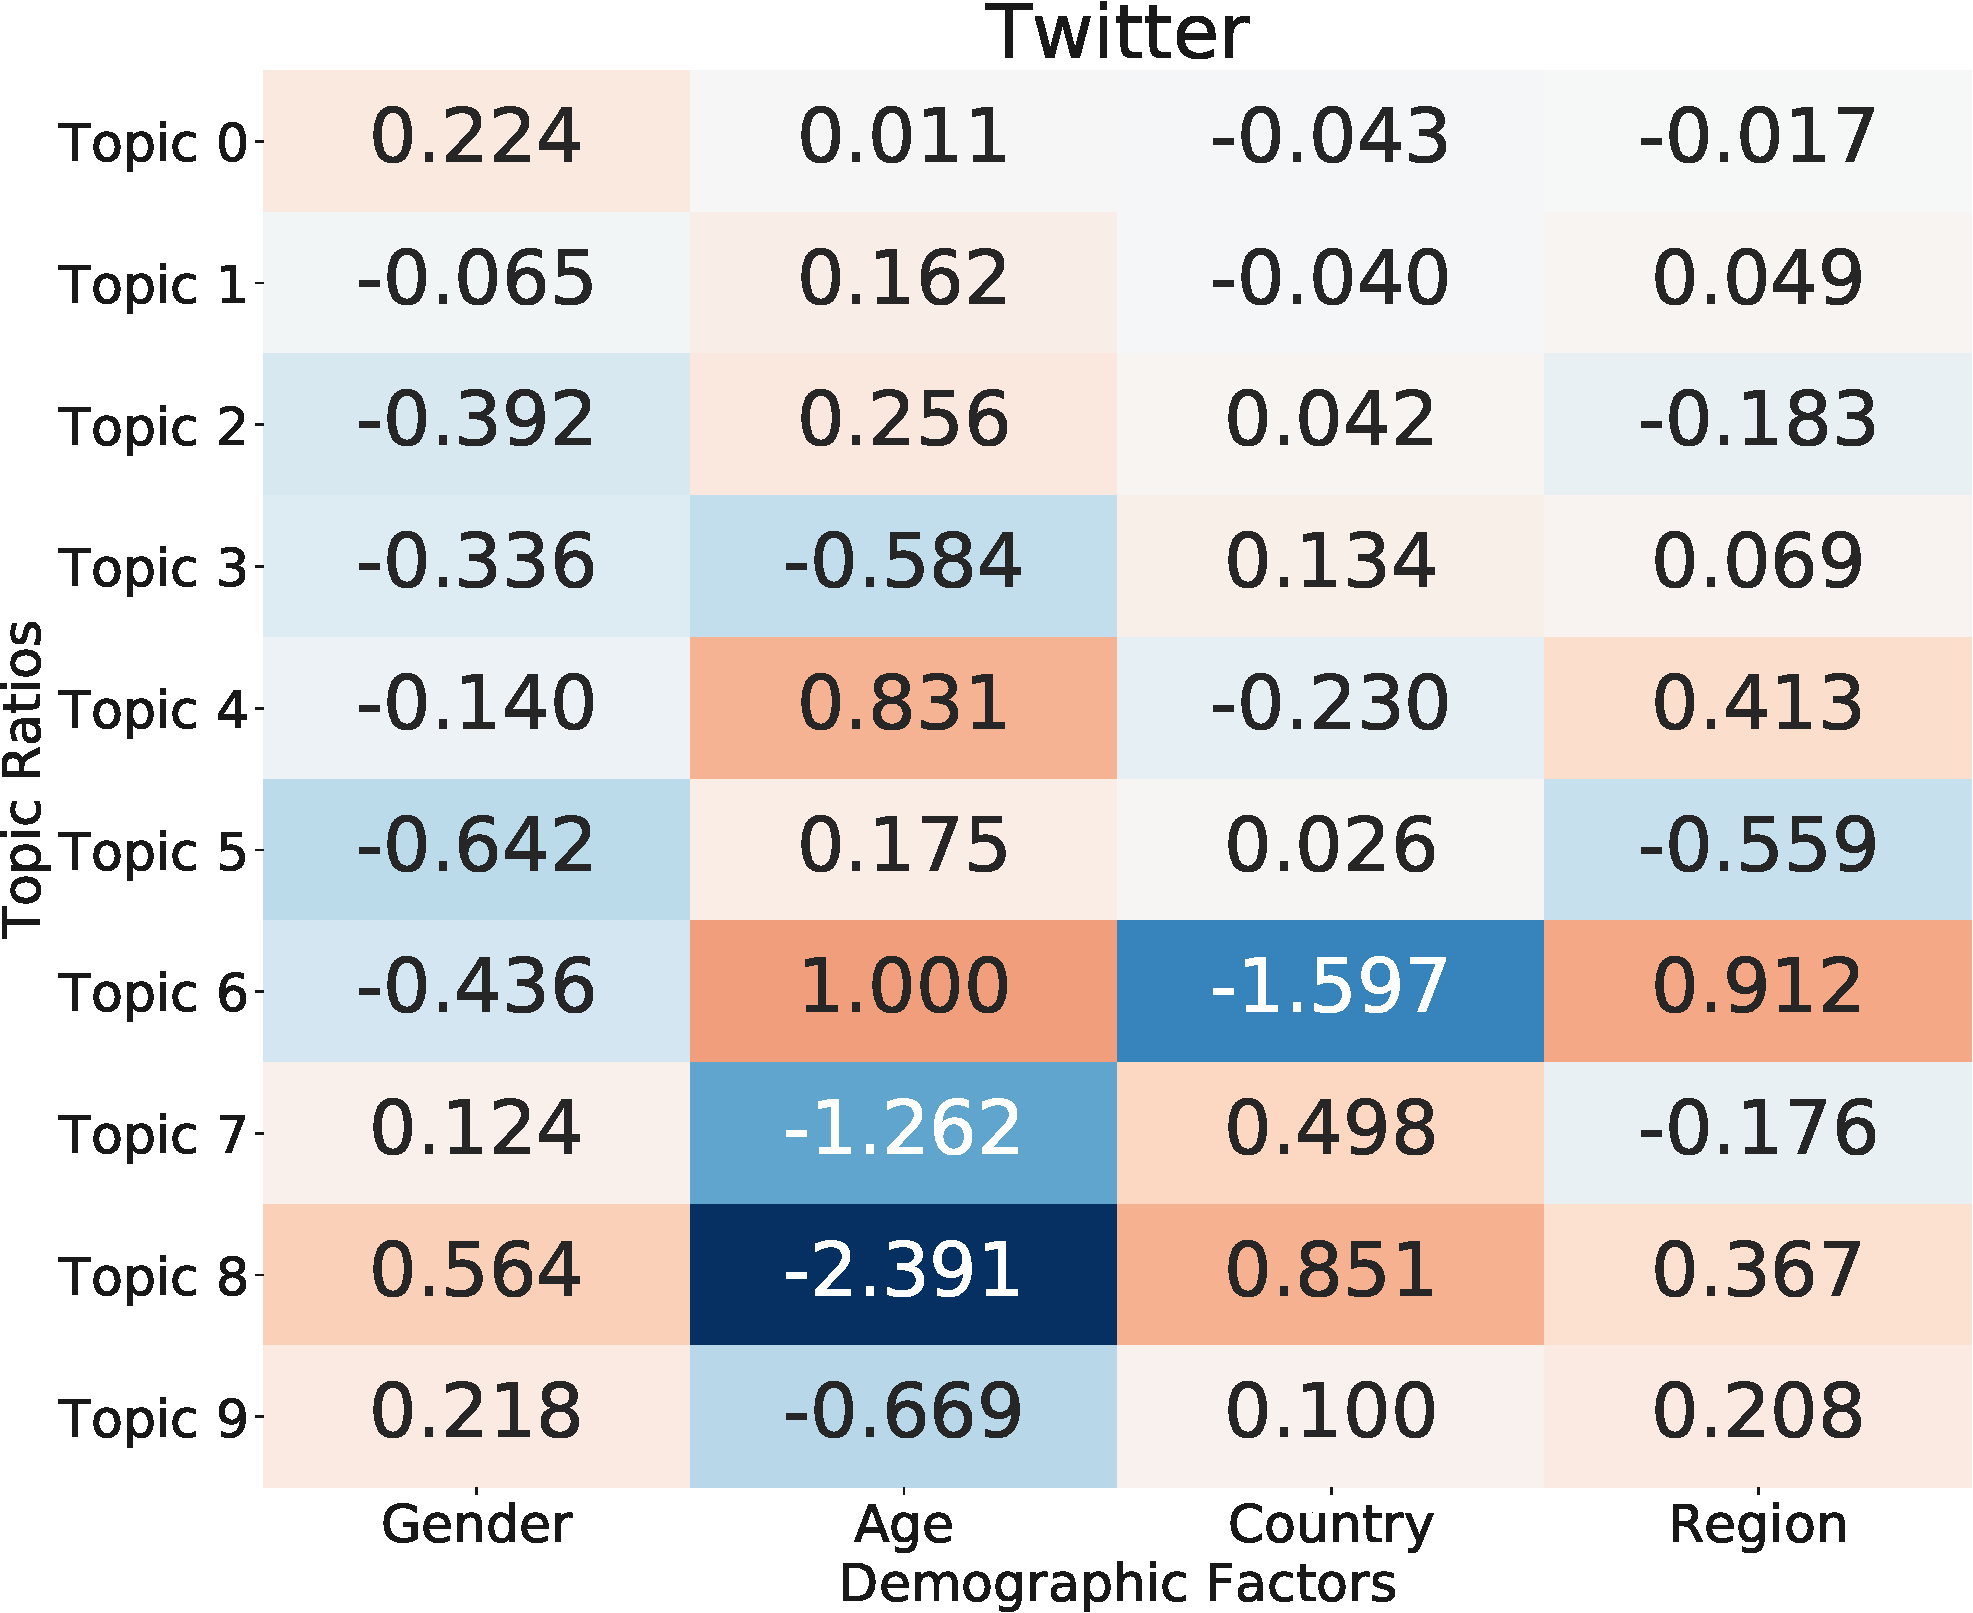
\includegraphics[width=0.49\textwidth]{./images/chapter4/twitter_ratio.pdf}
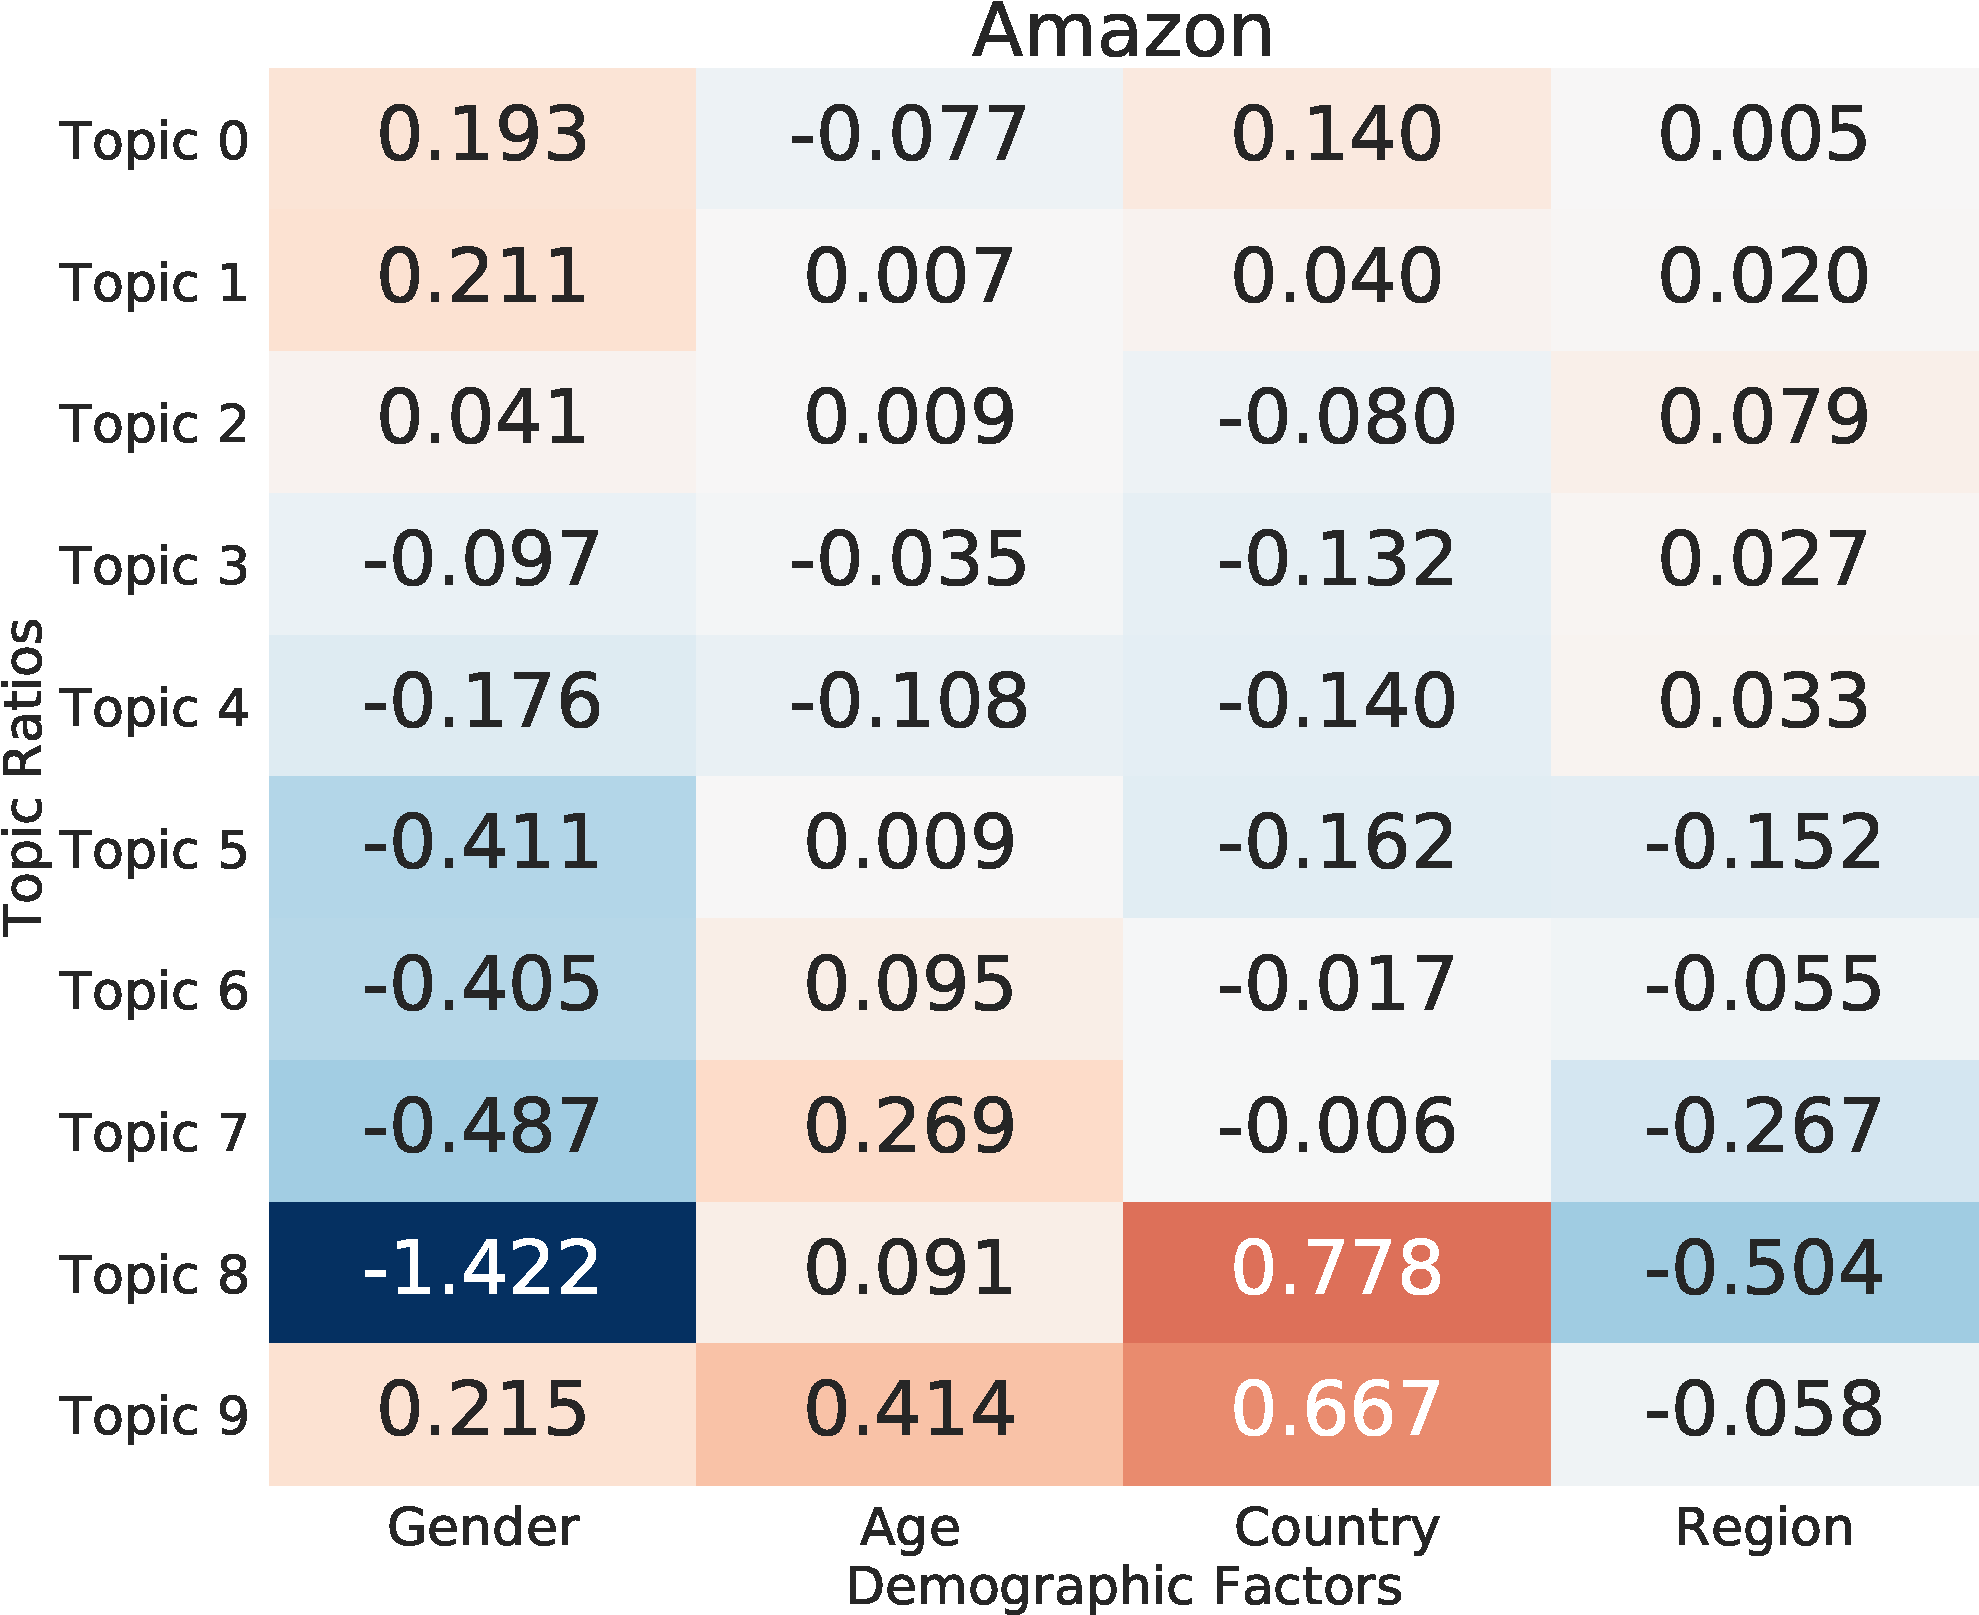
\includegraphics[width=0.49\textwidth]{./images/chapter4/amazon_ratio.pdf}
\newline
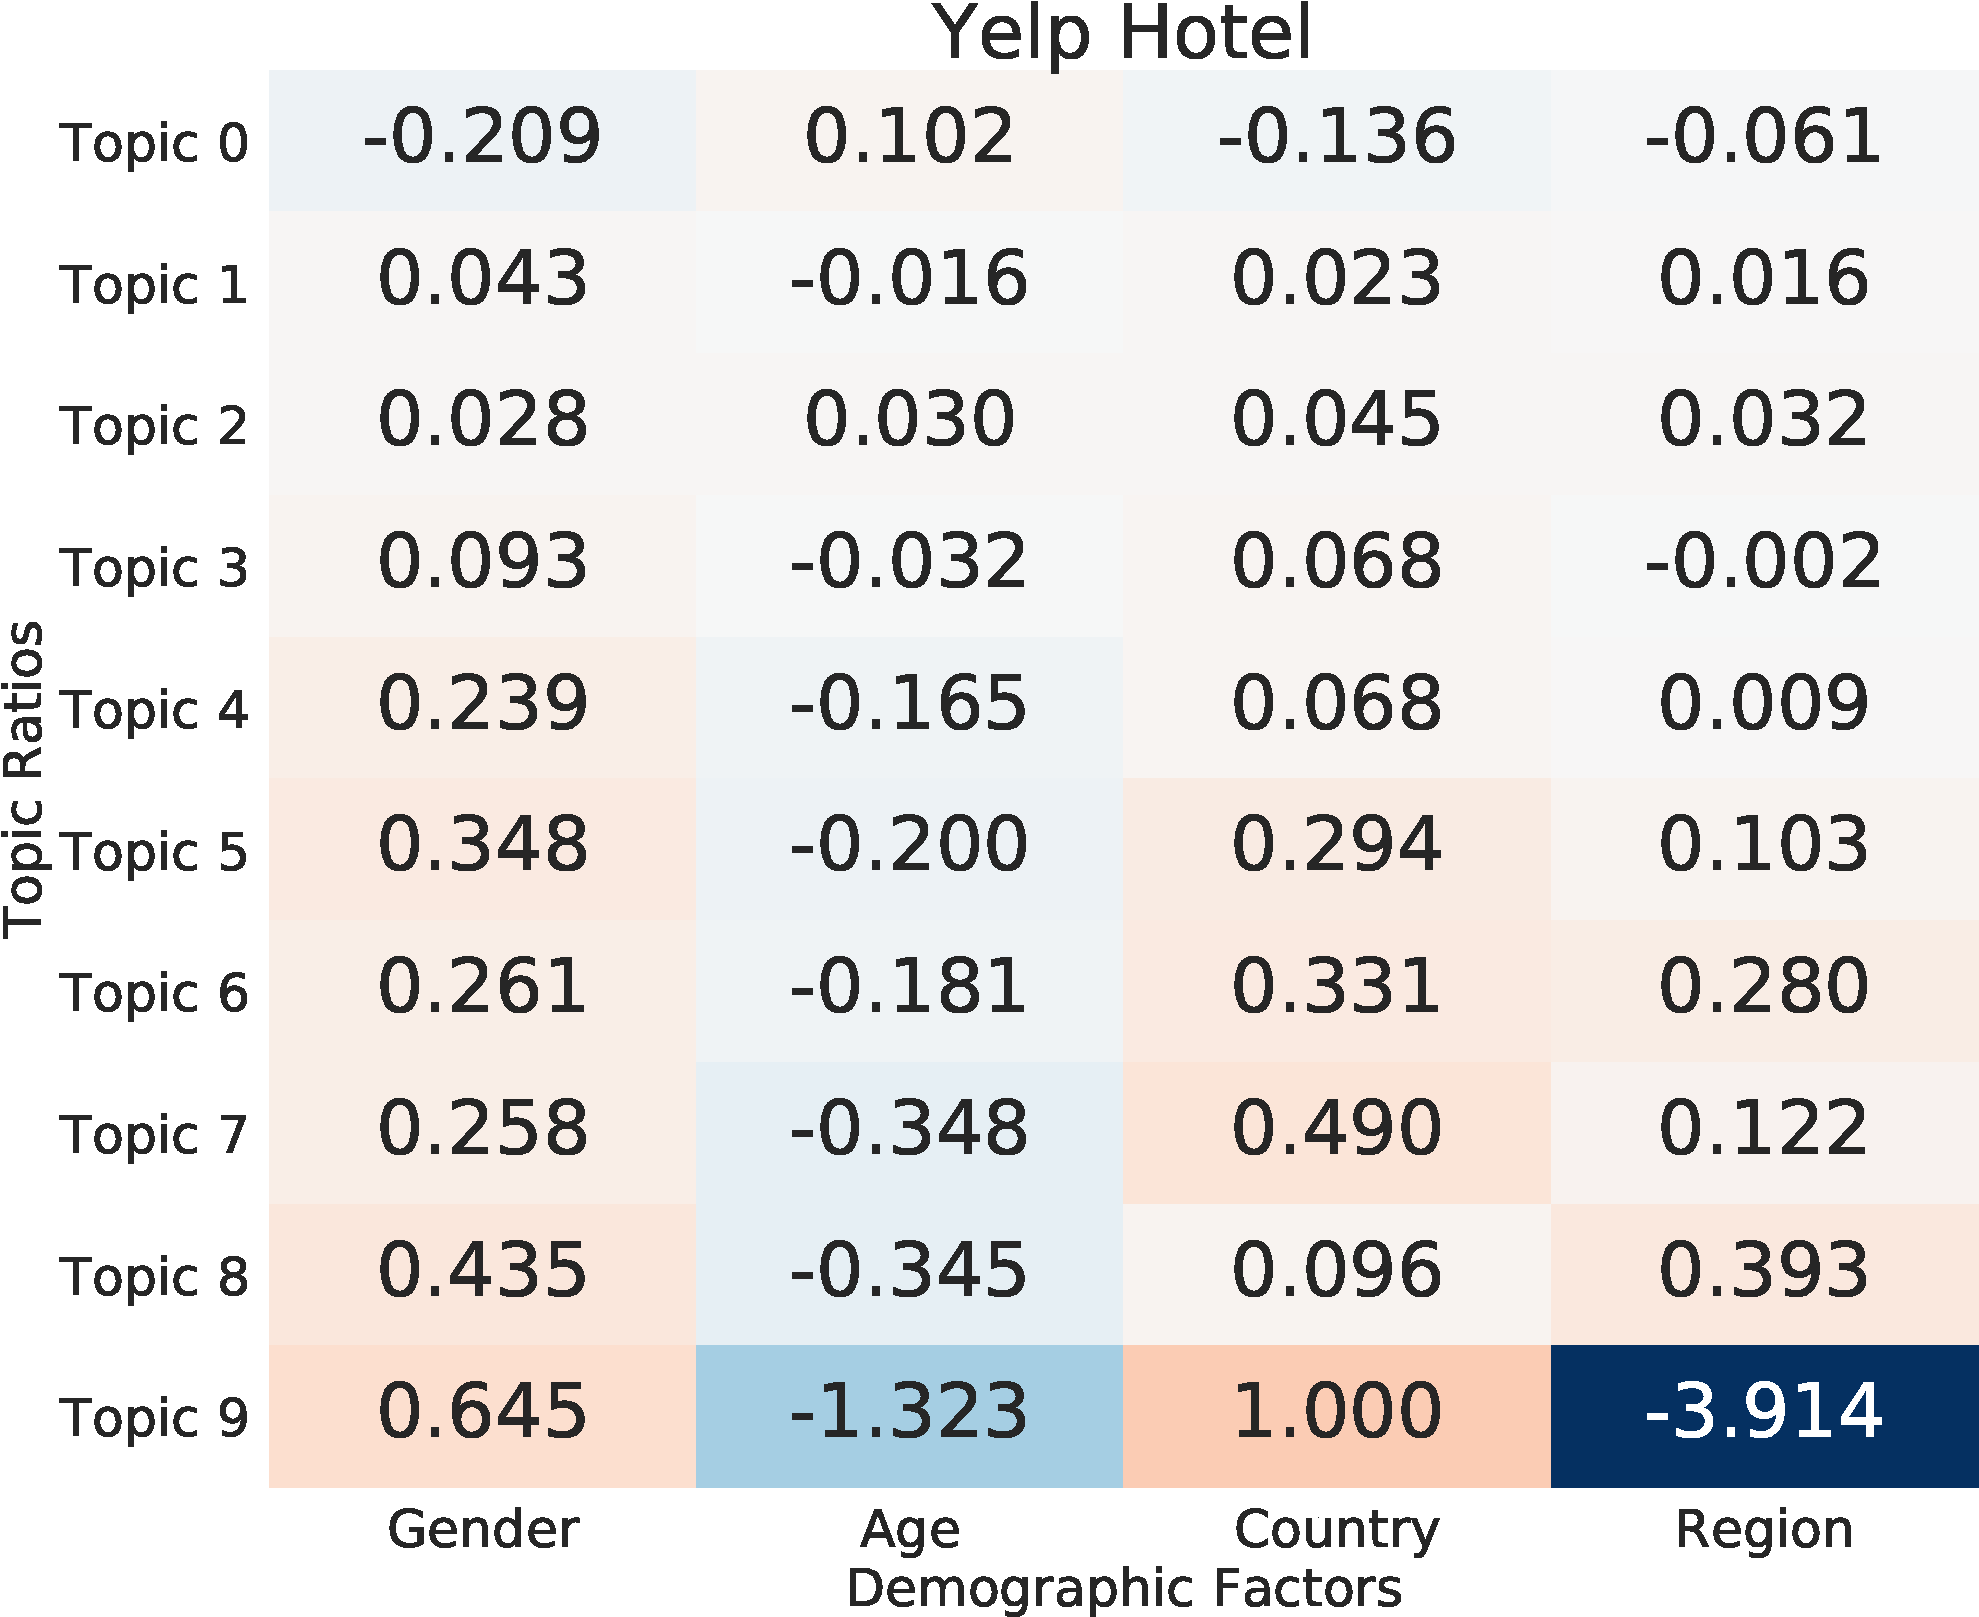
\includegraphics[width=0.49\textwidth]{./images/chapter4/yelp_hotel_ratio.pdf}
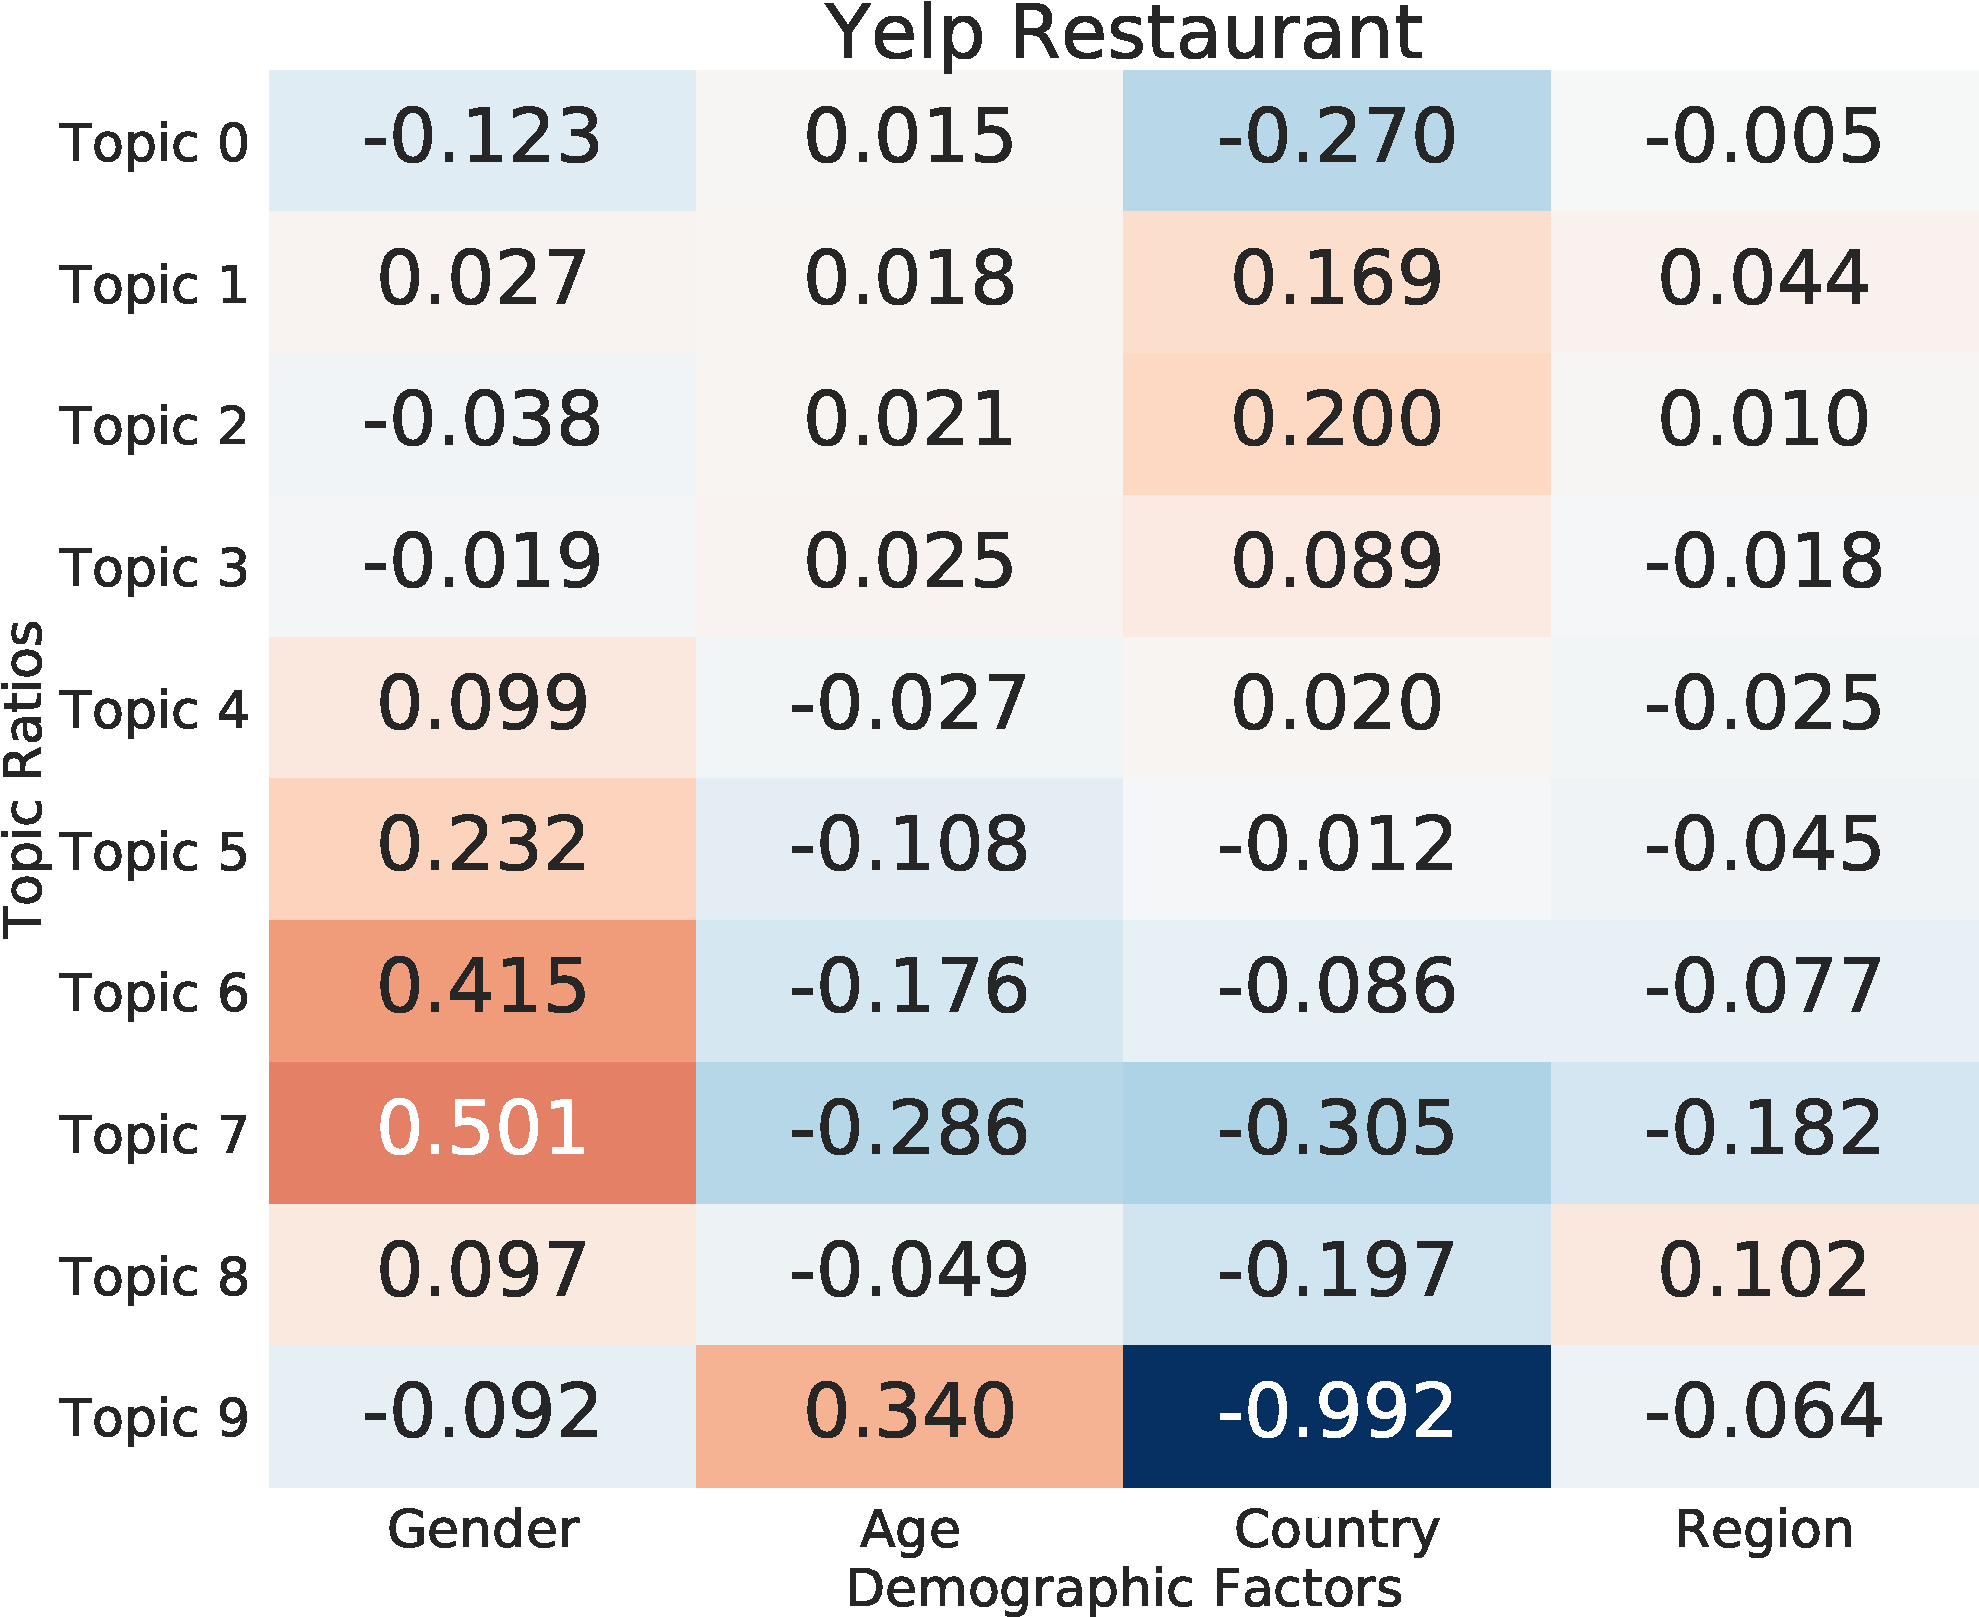
\includegraphics[width=0.49\textwidth]{./images/chapter4/yelp_rest_ratio.pdf}
\caption{Topic distribution log ratios. A value of 0 means that demographic groups use that topic in equal amounts, while values away from 0 mean that the topic is discussed more by one demographic group than the other group(s) in that factor.
}
\label{chap4:fig:vary}
\end{figure*}

We additionally examine how the distribution of text content varies across demographic groups. To characterize the content, we represent the text with a topic model.
We trained a Latent Dirichlet Allocation~\cite{blei2003latent} model with 10 topics using Gensim~\cite{rehurek2010software} with default parameters.
After training the topic model, each document $d$ is associated with a probability distribution over the 10 topics. 
The model learns a multinomial topic distribution $P(Z|D)$ from a Dirichlet prior, where $Z$ refers to each topic and $D$ refers to each document.
For each demographic group, we calculate the average topic distribution across the documents from that group.
Then within each factor, we calculate the log-ratio of the topic probabilities for each group.
For example, for topic $k$ for the gender factor,
we calculate $\log_2 \frac{P(Topic=k|Gender=\textrm{female})}{P(Topic=k|Gender=\textrm{male})}$.
The sign of the log-ratio indicates which demographic group is more likely to use the topic.
We do this for all factors;
for the region, we simply binarize the four values for this visualization (MW + W vs. NE + S).
Results are shown in Figure~\ref{chap4:fig:vary}.

The topic model was trained without removing stop words, in case stop word usage varies by group.
However, because of this, the topics all look very similar and are hard to interpret, so we do not show the topics themselves.
What we instead want to show is the degree to which the prevalence of some topics varies across demographic attributes, which are extracted independently from the text used to train the topic models.
We see that while most topics are fairly consistent across demographic groups, most datasets have at least a few topics with large differences:

\begin{itemize}
    \item \textbf{By gender} (G), $P(Z|D, G)$. Language styles are highly associated with the gender of online users~\cite{hovy2018capturing}. The Figure~\ref{chap4:fig:vary} shows there are obvious variations between male (left stacked bar) and female (right stacked bar). The Twitter topic distributions are more on the first topic. We infer the reason might be the data is highly focused on the ``flu vaccine''.
    \item \textbf{By age} (A), $P(Z|D, A)$. Some people change their linguistic styles as they age~\cite{wagner2012age}. We could partially confirm such a claim in our collected Twitter, Amazon and Yelp hotel data, which show more fluctuations of topic distributions. However, there are fewer variances in the Yelp restaurant data. 
    \item \textbf{By country} (C), $P(Z|D, C)$. From the third column of Figure~\ref{chap4:fig:vary}, we could observe that there are more significant variations in the Yelp restaurant data than other sources. It might be that people from different countries might express opinions in different ways. 
    \item \textbf{By region} (R), $P(Z|D, R)$. Goel et al.~\cite{goel2016social} show in online social media there are significantly different linguistic styles across different US regions. For example, due to English dialects among US regions, people in the Southern US use ``dese'' as ``these'' and people in Baltimore use ``ard'' as ``alright''. We might observe almost no variations in the Twitter data, which might be that people usually report ``flu vaccine'' in a similarly formal way. In contrast, we could observe that people talk more differently in the Amazon music data. 
\end{itemize}


\subsection{Are Document Categories Expressed Differently by Different User Groups?}

\begin{figure}[t!]
\centering
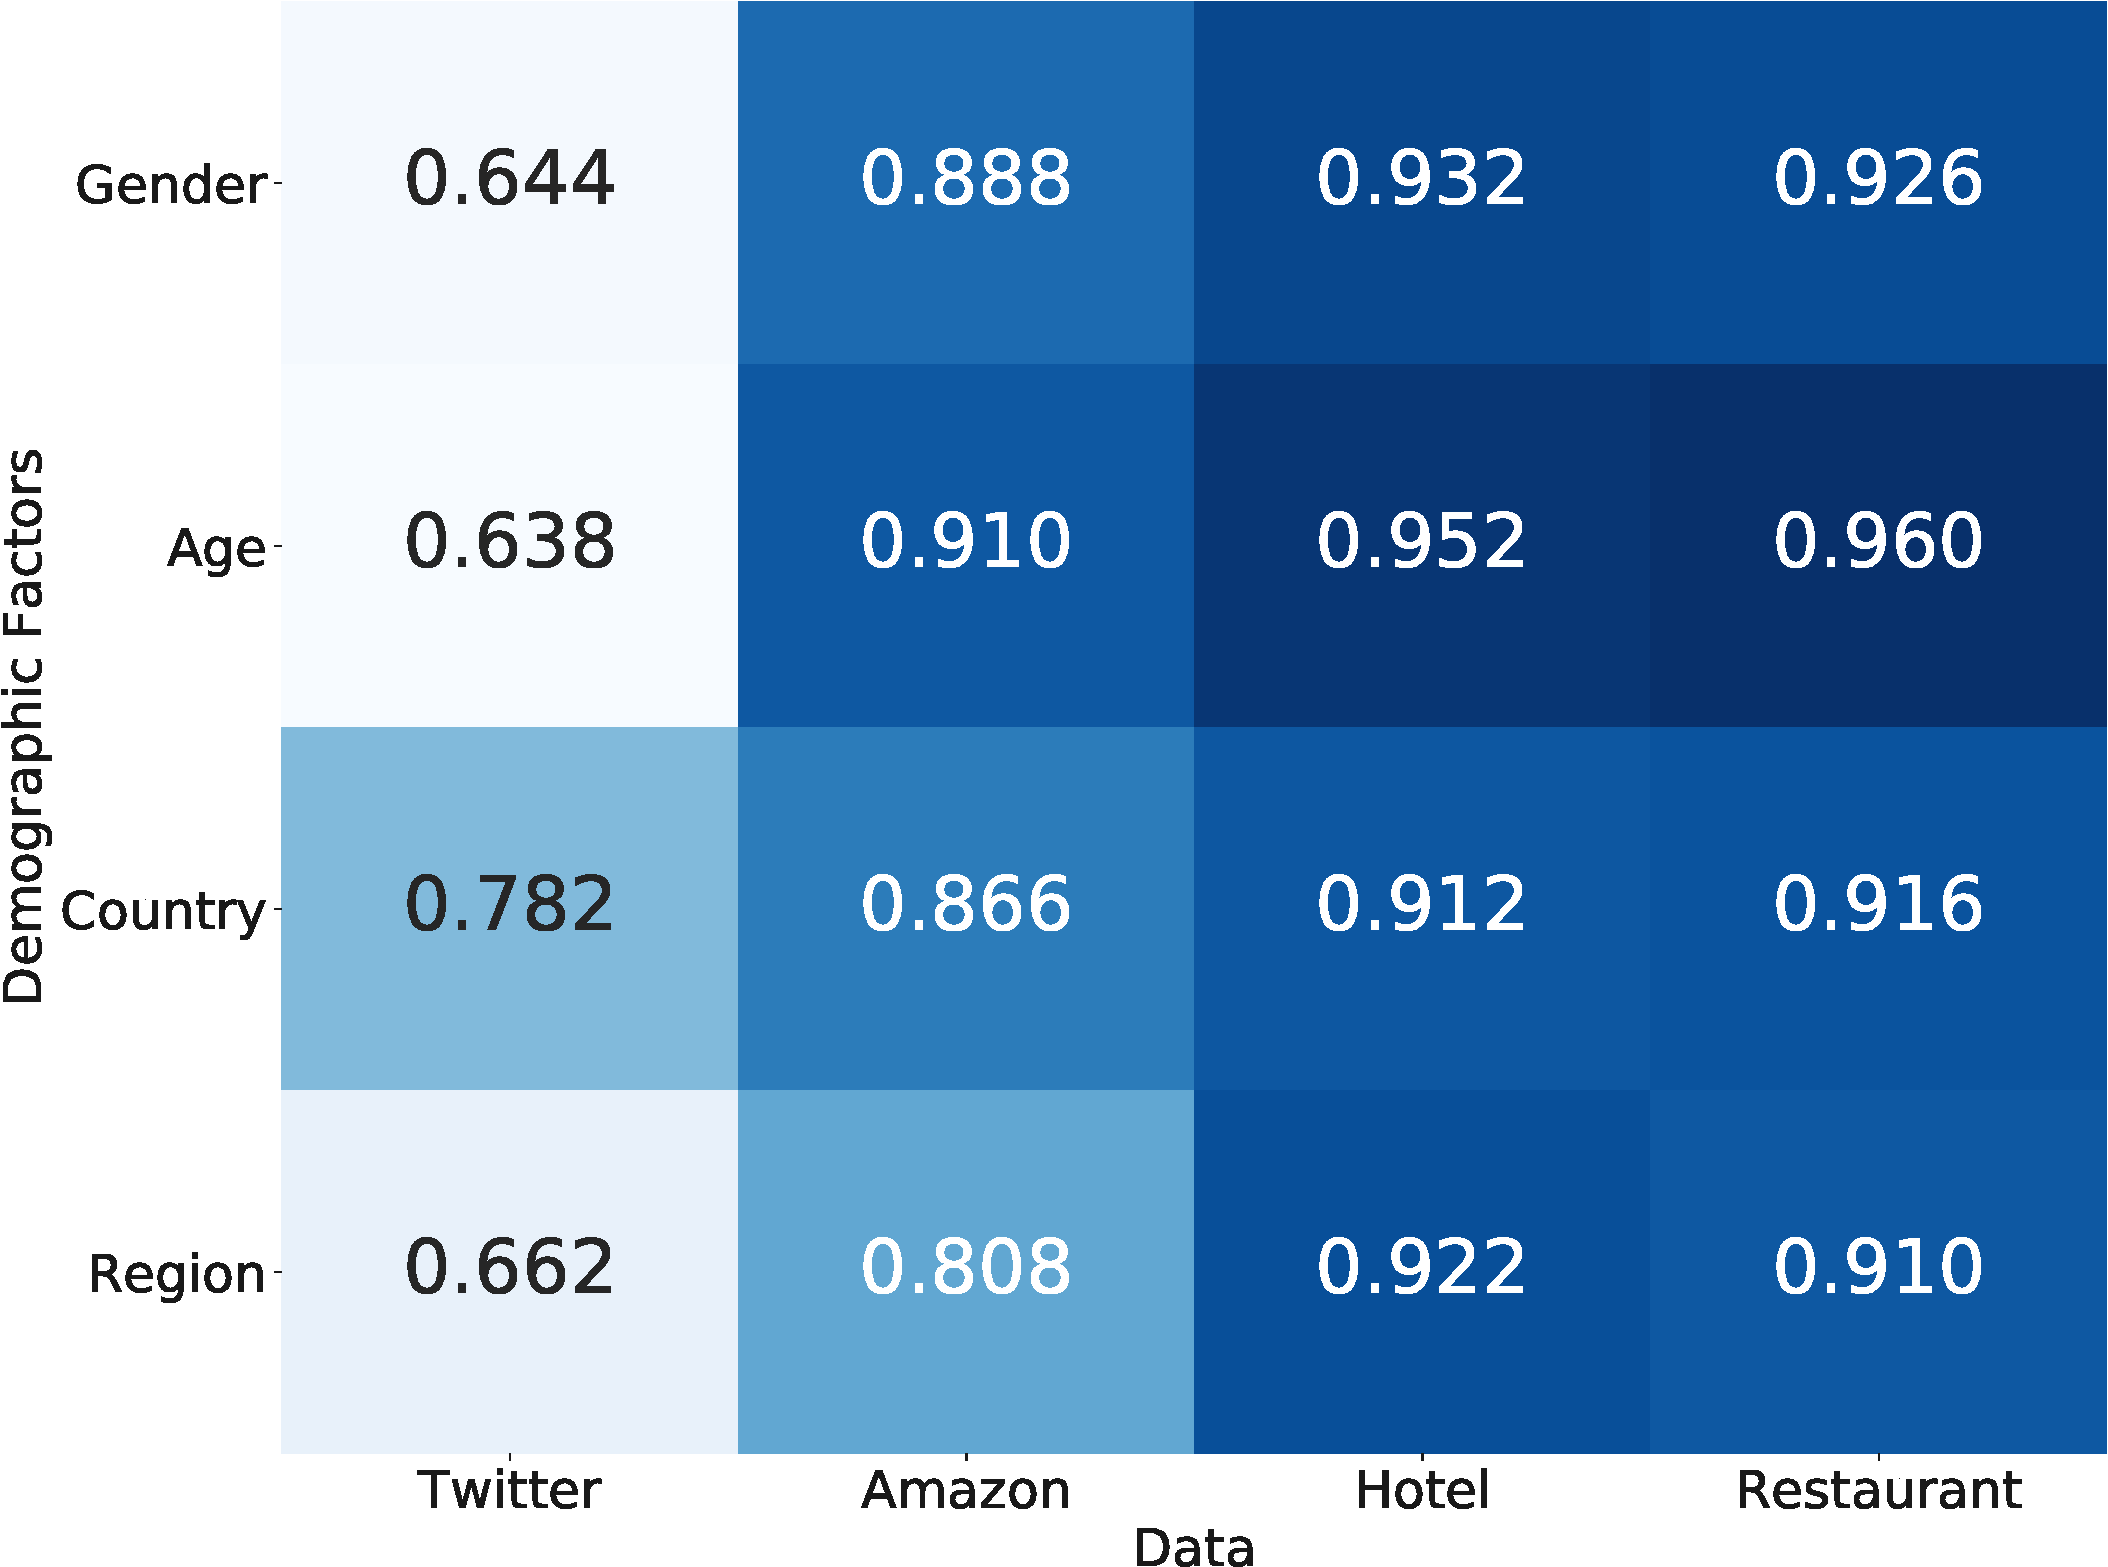
\includegraphics[scale=0.35]{./images/chapter4/overlap.pdf}
\caption{Overlap in most predictive classification features across different demographic groups, calculated for each demographic factor and each dataset. Darker color indicates less variation in word usage across demographic groups.
}
\label{chap4:fig:overlap}
\end{figure}

While text content varies across different user groups,
it is a separate question whether those variations will affect document classification.
For example, if men and women discuss different topics online,
but express sentiment in the same way,
then those differences will not affect a sentiment classifier.
Prior work has shown that the way 
people express opinions in online social media 
does vary by gender, age, geographic location and political orientation~\cite{hinds2018demographic};
thus, there is reason to believe that concepts like sentiment will be expressed differently by different groups.
As a final exploratory experiment,
we now consider whether the text features that are predictive of
document categories (e.g., positive or negative sentiment)
and vary with user factors.


To compare how word expressions vary among the demographic factors, we conduct a word-level feature comparison.
For each demographic group, we collect only documents that belong to that group and then calculate the n-gram features (same features as in Section~\ref{chap4:subsec:analysis}) that are most associated with the document class labels.
Using mutual information, we select the top 1,000 features for each attribute.
Then within each demographic factor (e.g., gender),
we calculate the percentage of the top 1,000 features that overlap across the different attribute values in that factor (e.g., male and female).
Specifically, if $S_0$ is the set of top features for one attribute and $S_1$ is the set of top features for another attribute, the percent overlap is calculated as $|S_0 \cap S_1|/1000$.
Results are shown in Figure~\ref{chap4:fig:overlap}. 
Lower percentages indicate higher variation in how different groups express the concepts being classified (e.g., sentiment).
The Twitter data shows the most variation while the Yelp hotel data shows the least variation.


\subsection{Model}
\label{chap4:subsec:model}

\begin{figure*}[htp]
\centering
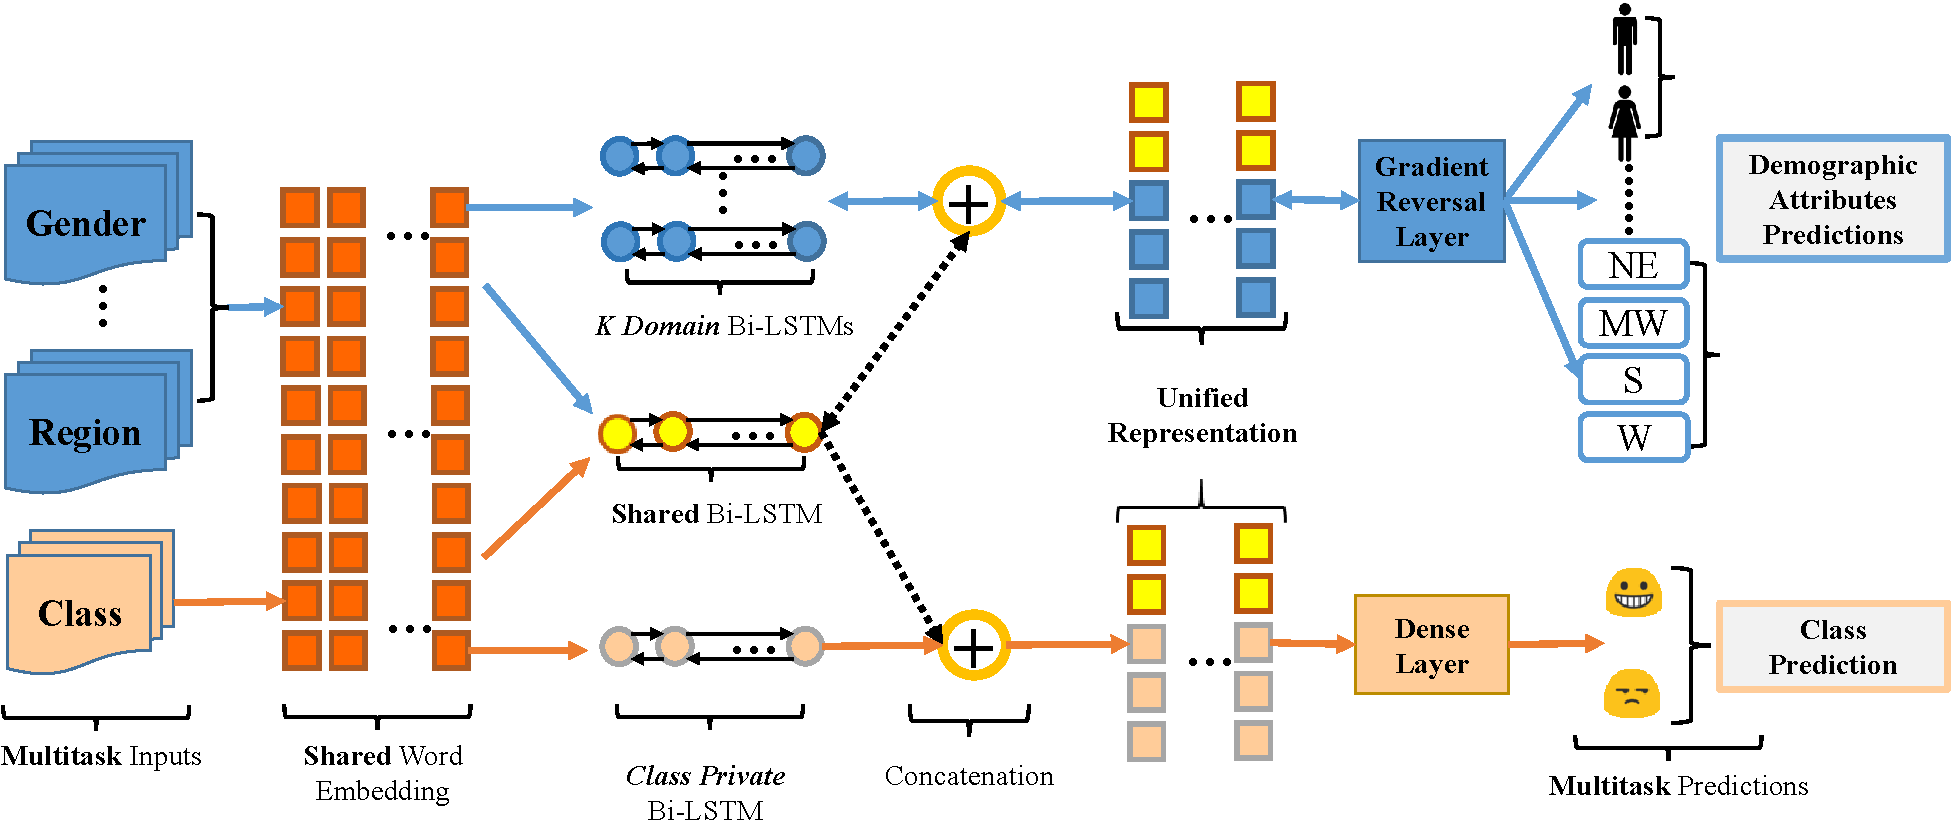
\includegraphics[width=1\textwidth]{./images/chapter4/model.pdf}
\caption{Neural User Factor Adaptation (NUFA) model. 
NUFA optimizes for two major tasks, demographic prediction (blue blocks and arrows) and text classification (light orange blocks and arrows). 
During the training phase, documents labeled with demographic information go through the demographic classifier, and documents with class labels go through the document classifier. 
This helps NUFA learn representations that are useful for classifying documents versus representations that are useful for predicting demographics.
At test time, documents are given only to the document classifier, leaving out the demographic classifiers.
}
\label{chap4:fig:model}
\end{figure*}

Models for user factor adaptation generally treat
this as a problem of {\em domain adaptation}~\cite{volkova2013exploring,lynn2017human}.
Domain adaptation methods are used to learn models that can be applied to data whose distributions may differ from the training data.
Commonly used methods include feature augmentation~\cite{daume2007frustratingly, joshi2013s, huang2018examining}
and structural correspondence learning~\cite{blitzer2006domain},
while recent approaches rely on 
domain adversarial training~\cite{ganin2016domain, chen2016adversarial, liu2017adversarial, huang2018modeling}. 
We borrow concepts of domain adaptation to construct a model that is robust to variations across user factors.


In our proposed {\bf Neural User Factor Adaptation (NUFA)} model, we treat each variable of interest (demographic attributes and document class label) as a separate but jointly modeled, prediction task.
The goal is to perform well at predicting document classes, while the demographic attribute tasks are modeled primarily for learning characteristics of demographic groups.
Thus, the model aims to learn discriminative features for text classification while learning to be invariant to the linguistic characteristics of demographic groups. 
Once trained, this classifier can be applied to test documents without requiring demographic attributes.

Concretely, we propose the multitask learning framework in Figure~\ref{chap4:fig:model}. 
The model extracts features from documents for the demographic attribute prediction and the classification tasks, as well as joint features for all tasks in which features for both demographics and document classes are mapped into the same vector space.
Each feature space is constructed with a separate Bidirectional Long Short-Term Memory model (Bi-LSTM)~\cite{hochreiter1997long}.

Because language styles vary across groups, as shown in Section~\ref{chap4:subsec:analysis}, information from each task could be useful to the other.
Thus, our intuition is that while we model the document and demographic predictions as independent tasks, the shared feature space allows the model to transfer knowledge from the demographic tasks to the text classification task and vice versa. 

However, we want to keep the feature space such that the features are predictive of document classes in a way that is invariant to demographic shifts. 
To avoid learning features for the document classifier that are too strongly associated with user factors, 
we use adversarial training.
The result is that the demographic information is encoded primarily in the features used for the demographic classifiers while learning invariant text features that work {\em across} different demographic groups for the document classifier. 

\paragraph{Domain Sampling and Model Inputs.} 
Our model requires all domains (demographic attributes) to be known during training, but not all attributes are known in our datasets.
Instead of explicitly modeling the missing data,
we simply sample documents where all user attributes of interest are available.
At test time, this limitation does not apply because only the document text is required as input to the document classifier.

We feed the inputs with all text documents. However, one issue with user demographic label in the real world is ``missing labels'', for example, a user might not provide any private information. Moreover, we could not do the same training steps proposed in the previous research~\cite{chen2016adversarial} that treats sampled training data as positive and test data as negative. Because they do not have a ``missing labels'' issue and in our scenario, demographic labels are well uniformly distributed in both training and test data. Therefore, we sample a batch of documents that have labels for each demographic prediction task. Noted that we only feed data to the document classifier during the test stage.

\paragraph{Shared Embedding Space.} 
We use a common embedding layer for both document and demographic factor predictions. The goal is that the trained embeddings will capture the language variations that are associated with the demographic groups as well as document labels. Parameters are initialized with pre-trained embeddings~\cite{mikolov2013distributed, pennington2014glove}.

\paragraph{K+2 Bi-LSTMs.} 
We combine ideas from two previous works on domain adaptation~\cite{liu2017adversarial, kim2017domain}. Kim et al.~\cite{kim2017domain} proposed $K$$+$$1$ Bi-LSTMs, where $K$ is the number of domains, and Liu et al.~\cite{liu2017adversarial} proposed to combine shared and independent Bi-LSTMs for each prediction task. In our model, we create one independent Bi-LSTM for each demographic domain (blue), one independent Bi-LSTM for the document classifier (orange), and one shared Bi-LSTM that is used in both the demographic prediction and document classification tasks (yellow). The intuition is to transfer learned information to one and the other through this shared Bi-LSTM while leaving some free spaces for both document label and demographic factors predictions. We then concatenate outputs of the shared LSTM with each task-independent LSTM together. This helps the text classifier capture demographic knowledge.

\paragraph{Demographic Classifier.} 
We adjust the degree to which the demographic classifiers can discriminate between attributes. 
To find a balance between the invariant knowledge and differences across user demographic factors, we apply domain adversarial training~\cite{ganin2016domain} (the blue block indicating the ``gradient reversal layer'') to each domain prediction task. The predictions use the final concatenated representations, where the prediction is modeled with a {softmax} function for the region and a binary {sigmoid} function for the other user demographic factors. 

\paragraph{Document Classifier.} 
We feed the concatenated outputs of the document and shared Bi-LSTMs to a single layer of the feed-forward network (the orange block indicating the ``dense layer''). Finally, the document classifier outputs a probability via a sigmoid.

\paragraph{Joint Multitask Learning.} 
We use the categorical cross-entropy loss to optimize the $K+1$ prediction tasks jointly. One question is how to assign importance to multiple tasks. Because our target is document classification, we assign a cost to the domain prediction loss ($L_{domain}$). Each prediction task has its own weight, $\alpha_k$. The final loss function is defined as $L = L_{doc} + \sum_{k=1}^K \alpha_k L_{domain, k}$. In summary, the proposed model learns and adapts to user demographic factors through three aspects: shared embeddings, shared Bi-LSTMs and joint optimization.


\subsection{Experiments}
\label{chap4:sec:dem_exp}
  
We experiment with document classification on our four corpora using various models. Our goal is to test whether models that adapt to user factors can outperform models that do not and to understand which components of models can facilitate user factor adaptation.
  
\subsubsection{Data Processing}

We replaced hyperlinks, usernames and hashtags with generic symbols. Documents were lowercased and tokenized using NLTK~\cite{bird2004nltk}. 
The corpora were randomly split into training (80\%), development (10\%) and test (10\%) sets.
We train the models on the training set and find the optimal hyperparameters on the development set. We randomly shuffle the training data at the beginning of each training epoch. The evaluation metric uses the weighted F1 score.

%
%\begin{table}[ht]
%  \centering
%  \resizebox{\columnwidth}{!}{
%    \begin{tabular}{c|ccc|c}
%     \hline\hline
%     Datasets & Train & Dev. & Test & Total\\
%     \hline
%     Twitter & 7,875 & 984 & 985 & 9,844 \\
%     Amazon & 32,335 & 4,042 & 4,042 & 40,419 \\
%     Hotel & 135,164 & 16,896 & 16,896 & 168,956 \\
%     Restaurant & 570,750 & 71,344 & 71,344 & 713,438 \\
%     \hline
%    \end{tabular}
%    }
%    \caption{Data statistics.}
%    \label{chap4:table:statics}
%\end{table}
%
%%

\subsubsection{No Adaptation Baselines}
We compare to three standard classifiers that do not perform adaptation.

\paragraph{N-gram.} We extract TF-IDF-weighted features of 1-, 2- and 3-grams on the corpora, using the most frequent 15K features with the minimum feature frequency as 2.
We trained a logistic regression classifier using the \texttt{SGDClassifier} implementation in scikit-learn~\cite{pedregosa2011scikit}
using a batch size of 256 and 1,000 iterations. 

\paragraph{CNN.} 
We used Keras~\cite{chollet2015keras} to implement the Convolutional Neural Network (CNN) classifier described in~\cite{kim2014convolutional}. To keep consistent, we initialize the embedding weight with pre-trained word embeddings~\cite{mikolov2013distributed,pennington2014glove}. We only keep the 15K most frequent words and replace the rest with an ``unk'' token. Each document was padded to a length of 50. We fed 50 documents to the model each batch and trained for 20 epochs.

\paragraph{Bi-LSTM.} We build a bi-directional Long Short Term Memory (bi-LSTM)~\cite{hochreiter1997long} classifier. The classifier is initialized with the pre-trained word embeddings, and we initialize training with the same parameters used for the NUFA.


\subsubsection{Adaptation Models}

We consider two domain adaptation models as our baselines that can adapt for user factors, a non-neural method and a neural model.
We then provide the training details of our proposed model, NUFA.
Finally, we consider two variants of NUFA that ablate components of the model, allowing us to evaluate the contribution of each component.

\paragraph{FEDA.} 
Lynn et al.~\cite{lynn2017human} used a modification of the ``frustratingly easy'' domain adaptation (FEDA) method~\cite{daume2007frustratingly} to adapt for user factors. 
We use a modification of this method where the four user factors and their values are treated as domains.
We first extract domain-specific and general representations as TF-IDF-weighted n-gram (1-, 2, 3-grams) features. We extract the top 15K features for each domain and the general feature set.
With this method, the feature set is augmented such that each feature has a domain-specific version of the feature for each domain, as well as a general domain-independent version of the feature.
The features values are set to the original feature values for the domain-independent features and the domain-specific features that apply to the document, while domain-specific features for documents that do not belong to that domain are set to $0$.
For example, using gender as a domain, a training document with a female author would be encoded as $[F_{general}, F_{domain, female}, 0]$, while a document with a male author would be encoded as $[F_{general}, 0, F_{domain, male}]$.
Different from prior work with FEDA for user-factor adaptation, 
at test time we only use the general, domain-independent features;
the idea is to learn a generalized feature set that is domain invariant.
This is the same approach we used in recent work using FEDA to adapt classifiers to temporal variations~\cite{huang2018examining}.


\paragraph{DANN.} We consider the domain adversarial training network~\cite{ganin2016domain} (DANN) on the user factor adaptation task. We use Keras to implement the same network and deploy the same pre-trained word embeddings as in NUFA. We then set the domain prediction with the demographic factors prediction and keep the document label prediction as the default. We train the model with 20 epochs with a batch size of 64. Finally, we use the model at the epoch when the model achieves the best result on the development set for the final model.


\paragraph{NUFA.}
We initialize the embedding weights by the pre-trained word embeddings~\cite{mikolov2013distributed, pennington2014glove} with 200-dimensional vectors. All LSTMs are fixed outputs as 200-dimension vectors. We set the dropout of LSTM training to 0.2 and the flip gradient value to .01 during the adversarial training. The dense layer has 128 neurons with a ReLU activation function and a dropout of 0.2. User factors and document label predictions are optimized jointly using Adam~\cite{kingma2014adam} with a learning rate of 0.001 and a batch size of 64. We train NUFA for up to 20 epochs and select the best model on the development set. 
For single-factor adaptation (next section), we set $\alpha$ to 0.1;
for multi-factor adaptation, we use a heuristic for setting $\alpha$ described in that section.
We implemented NUFA in Keras~\cite{chollet2015keras}.

\paragraph{NUFA--s.} 
To understand the role of the shared Bi-LSTM in our model, we conduct experiments on NUFA without the shared Bi-LSTM. We follow the same experimental steps as NUFA and denote it as NUFA$-$s (NUFA minus shared Bi-LSTM). 

\paragraph{NUFA--a.} 
To understand the role of the adversarial training in our model, we conduct experiments of the NUFA without adversarial training, denoted as NUFA$-$a (NUFA minus adversarial).


\subsubsection{Results}


\begin{table}[t!]
\centering
\begin{tabular}{c|c|c|c|c}
 & Twitter & Amazon & Hotel & Rest. \\\hline
 \multicolumn{5}{c}{No Adaptation} \\\hline
N-gram & .866 & .793 & .857 & .866 \\
CNN & .879 & .776 & .825 & .846 \\
Bi-LSTM & .869 & .776 & .842 & .875 \\\hline
\multicolumn{5}{c}{Adaptation (Gender)} \\\hline
FEDA & .814 & .809 & \textbf{.865} & .874 \\
DANN & .864 & .832 & .813 & .855 \\ \hline
NUFA$-$s & .880 & \em .845 & .857 & .869 \\
NUFA$-$a & .874 & .842 & .852 & .868 \\
NUFA & \em .886 & .844 & .854 & \textbf{.881} \\ \hline
\multicolumn{5}{c}{Adaptation (Age)} \\\hline
FEDA & .813 & .801 & \bf .865 & .873 \\
DANN & .856 & .824 & .811 & .851 \\ \hline
NUFA$-$s & .872 & \em .843 & .850 & .879 \\
NUFA$-$a & .882 & .841 & .852 & .878 \\
NUFA & \em .885 & .839 & .857 & \em .880 \\ \hline
\multicolumn{5}{c}{Adaptation (Country)} \\\hline
FEDA & .826 & .768 & \bf .865 & .877 \\
DANN & .868 & .828 & .827 & .855 \\ \hline
NUFA$-$s & .882 & \em .844 & .854 & \em .879 \\
NUFA$-$a & .880 & .838 & .855 & .877 \\
NUFA & \textbf{.896} & .843 & .854 & \em .879 \\ \hline
\multicolumn{5}{c}{Adaptation (Region)} \\\hline
FEDA & .826 & .780 & \em .864 & .869 \\
DANN & .875 & .825 & .823 & .852 \\\hline
NUFA$-$s & .874 & .833 & .854 & .878 \\
NUFA$-$a & .882 & .838 & .854 & .875 \\
NUFA & \em .893 & \textbf{.848} & .853 & \em .880\\ \hline
\end{tabular}
\caption{Performance (weighted F1) of no adaptation and single user factor adaptation.
For each dataset, the best score within each demographic domain is italicized; the best score overall is bolded.
}
\label{chap4:table:single}
\end{table}

\paragraph{Single-Factor Adaptation.} We first consider user factor adaptation for each of the four factors individually. 
Table~\ref{chap4:table:single} shows the results.
Adaptation methods almost always outperform the non-adaptation baselines;
the best adaptation model outperforms the best non-adaptation model by $1.5$ to $5.5$ points. 
The improvements indicate that adopting the demographic factors might be beneficial for the classifiers. User factor adaptation thus appears to be important for text classification. 

Comparing the adaptation methods,
our proposed model (NUFA) is best on three of four datasets.
On the Hotel dataset, the n-gram model FEDA is always best;
this seems to be a dataset where neural methods perform poorly, since even the n-gram baseline with no adaptation often outperformed the various neural models. 
Whether a neural model is the best choice depends on the dataset,
but among the neural models, NUFA always outperforms DANN.
Finally, the full NUFA model most often outperforms the variants without the shared Bi-LSTM (NUFA$-$s) and without adversarial training (NUFA$-$a). 


\paragraph{Multi-Factor Adaptation.} We experiment with adapting to all four user factors together.
Recall that each domain prediction task in NUFA is weighted by $\alpha_k$.
Initially, we simply used a uniform weighting, $\alpha_k = \alpha/K$,
but we find that we can improve performance with non-uniform weighting.
Because optimizing the $\alpha$ vector would be expensive, 
we instead propose a heuristic that weighs the domains
based on how much each domain is expected to influence the text.
We define $\alpha_k = s_k / (\sum_{k'} s_{k'})$, where $s_k$ is the F1 score of demographic attribute prediction for domain $k$ from Table~\ref{chap4:table:explo}.
We denote this method as {\bf NUFA+w}, which refers to this additional weighting process.

\begin{table}[htp]
\centering
\begin{tabular}{c|c|c|c|c}
 & Twitter & Amazon & Hotel & Rest. \\\hline
\multicolumn{5}{c}{Baseline Adaptation} \\\hline
FEDA & .806 & .778 & \bf .867 & .869 \\\hline
DANN & .880 & .828 & .830 & .858 \\\hline
\multicolumn{5}{c}{Proposed Model} \\\hline
NUFA & .887 & .848 & .853 & .879 \\
NUFA+w & \bf .901 & \bf .852 & .855 & \bf .885 \\
\end{tabular}
\caption{Results of adaptation for all four user factors.}
\label{chap4:table:multi}
\end{table}

Table~\ref{chap4:table:multi} shows that combining all user factors
provides a small gain over single-factor adaptation;
the best multi-factor result is higher than the best single-factor result for each dataset.
As with single-factor adaptation, FEDA works best for the Hotel datasets,
while NUFA+w works best for the other three.
Without adding weighting to NUFA, the multi-factor performance is comparable to single-factor performance;
thus, task weighting seems to be critical for good performance when combining multiple factors.


\section{User Factor Adaptation -- User Interests}
\label{chap4:sec:uemb}

The previous Section~\ref{chap4:sec:daa} explored language variations across user demographic groups and proposed a method to adapt user demographic attributes into neural document classifiers via a multitask learning framework.
In this section, we will present the second user factor adaptation method by using multitask user embedding, which jointly learns user behaviors and interests from posts.

User embedding, which is to learn a fixed-length representation based on multiple user posts for each user, can infer the user latent information into a unified vector space~\cite{benton2018learning, pan2019social}.
The inferred latent representations from online content can be predictive towards user demographic attributes~\cite{volkova2015inferring, wang2018cross, farnadi2018user, lynn2020hierarchical} and behaviors~\cite{amir2017quantifying, benton2017multitask, ding2017multi}.
By treating user embeddings as global contexts, research can combine the contexts with document representations, personalize document classification models, and further improve model performance~\cite{tang2015learning, chen2016neural, yang2017overcoming, wu2018improving, zeng2019joint, huang2019deep}.
The semantic variations across users can help models better understand online documents from a high level.

However, existing user embedding methods \cite{amir2016modelling, benton2016learning, xing2017incorporating, pan2019social} mainly focus on extracting features from language itself while ignoring user interests such as topics of posted documents, types of purchased items and genres of watched movies.
Promising recent research has demonstrated that the user factor can further improve user demographic attribute prediction \cite{farnadi2018user} and sentiment analysis \cite{yang2017overcoming}.
\cite{lynn2017human} treated the language variations as a domain adaptation problem and referred to this idea as \textit{user factor adaptation}.

In this section, we propose a multitask framework to model the language variations and incorporate the user factor into user embeddings.
We focus on three online review datasets from Amazon, IMDb and Yelp, which contain diverse user interests in shopping behaviors.

We first explore how the user factor, user interests, can cause language and classification variations in Section~\ref{chap4:subsec:analysis}.
We then propose our user embedding model that adapts the hidden user factor using a multitask learning framework in Section~\ref{chap4:subsec:model2}.
The current research~\cite{pan2019social} generally evaluates the user embedding via downstream tasks where the user annotations are hard to obtain. 
For example, the MyPersonality~\cite{kosinski2015facebook} that was used in previous work~\cite{ding2017multi, farnadi2018user, pan2019social} is no longer available. 
Research suggests that the intrinsic evaluation including clustering is better than the extrinsic evaluation including the text classification~\cite{schnabel2015evaluation}.
Our proposed intrinsic approach can provide a new perspective for future user embedding evaluation.


\subsection{Data}
\label{chap4:subsec:data2}

We collected English reviews of Amazon (health product), IMDb and Yelp from the publicly available sources~\cite{he2016ups, yelp_2019, imdb2020dataset}.
For the IMDb dataset, we crawled movie and user metadata of review documents, including user historical reviews, user profiles, movie profiles, etc.\footnote{We included English movies produced in the US from 1960 to 2019.}
Each review associates with its author and the corresponding \textit{product}, which refers to a movie in the IMDb data, a business unit in the Yelp data and an item in the Amazon data.
To keep consistency in each dataset, we keep the top 4 popular genres of products and the review documents with no less than 10 tokens.\footnote{The top 4 product categories of Amazon-health, IMDb and Yelp are [sports nutrition, sexual wellness, shaving \& hair removal, vitamins \& dietary supplements], [comedy, thriller, drama, action] and [restaurants, health \& medical, home services, beauty \& spas] respectively.}
We dropped non-English review documents by the language detector~\cite{lui2012langid}, lowercased all tokens in the datasets and tokenized the corpora using NLTK~\cite{bird2004nltk}.
The review datasets have different score scales, and therefore we encode each review score into three discrete categories: positive ($>3$ for the Yelp and Amazon, $>6$ for the IMDb), negative ($<3$ for the Yelp and Amazon, $<5$ for the IMDb) and neutral.


To protect user privacy, we anonymize all user-related information even though our datasets were completely from publicly available sites. 
We only store datasets necessary for this study and do not release any private information associated with individual profiles.
Table~\ref{chap4:tab:data2} shows a summary of the datasets.


\begin{table*}[htp]
\centering
% \resizebox{0.90\textwidth}{!}{
    \begin{tabular}{c||cccc||ccc}
    Data & Users & Docs & Products & Tokens & Train & Dev & Test \\\hline\hline
    Amazon-Health & 11,438 & 80,592 & 3,822 & 127 & 64,474 & 8,060 & 8,061 \\
    IMDb & 6,089 & 123,184 & 642 & 187 & 98,548 & 12,319 & 12,320 \\
    Yelp & 76,323 & 551,695 & 9,327 & 152 & 441,357 & 55,170 & 55,171 \\
    \end{tabular}
% }
\caption{Statistical summary of the Amazon, Yelp and IMDb review datasets. Amazon-health refers to health-related reviews. Tokens mean average tokens per document. We present the data split for the evaluation task of text classification on the right side.}
\label{chap4:tab:data2}
\end{table*}



\subsection{Exploratory Analysis of User Variations}

Language varies across user factors such as user interests \cite{oba2019modeling}, demographic attributes \cite{huang2019neuraluser}, social relations \cite{yang2017overcoming}.
In this section, our goal is to quantitatively analyze whether the user interests cause the user language variations, which can reduce the effectiveness and robustness of user embeddings.
We approach this by two analysis tasks, first by measuring word feature similarity based on user interests, and second by examining how classifier performance depends on the grouped user interests in which the model is trained and applied.



\subsubsection{Word Usage Variations}

\begin{figure*}[t]
    \centering
    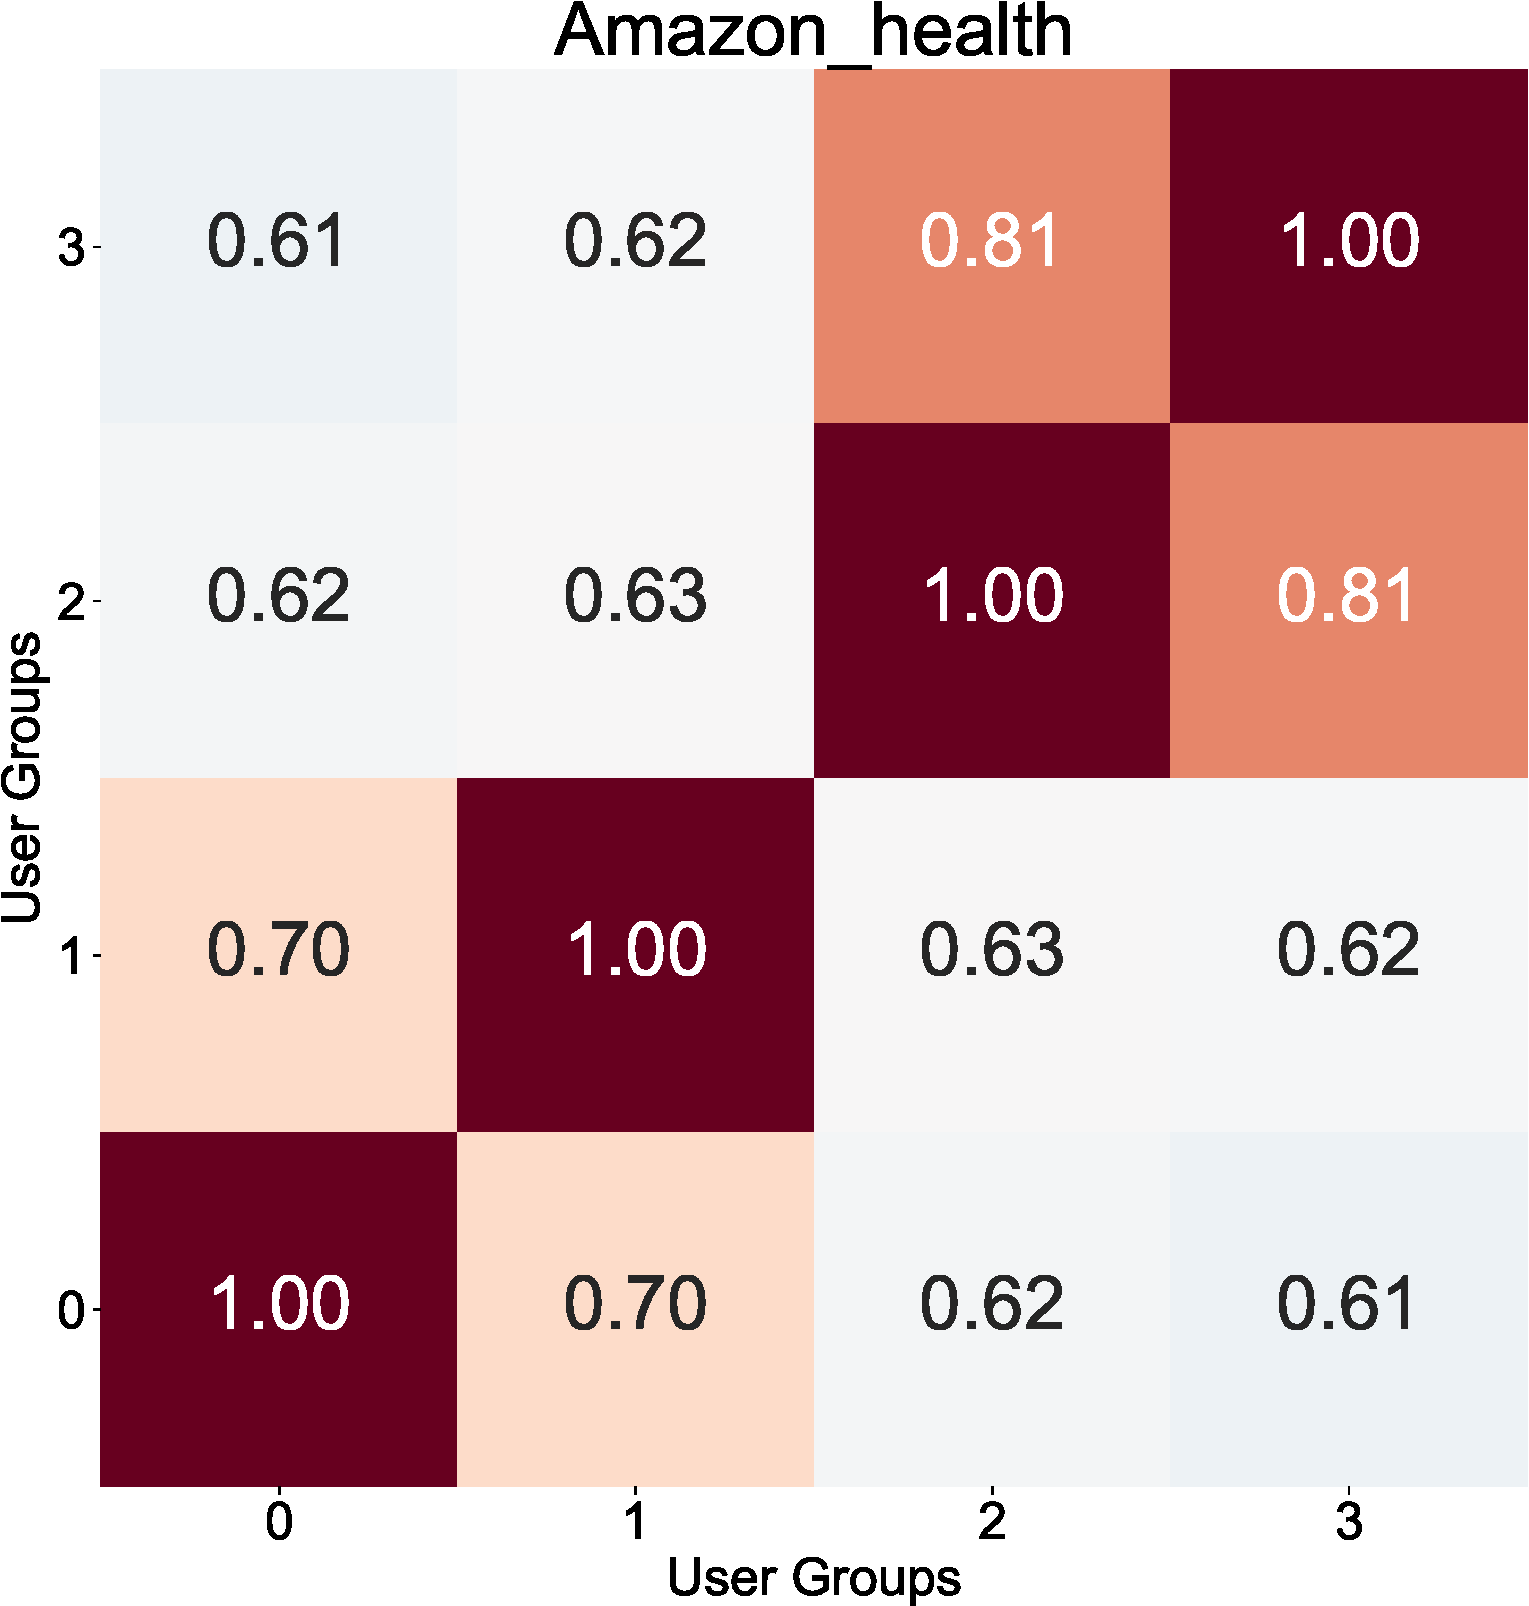
\includegraphics[width=0.325\textwidth]{./images/chapter4/uembedding/amazon_health_word.pdf}
    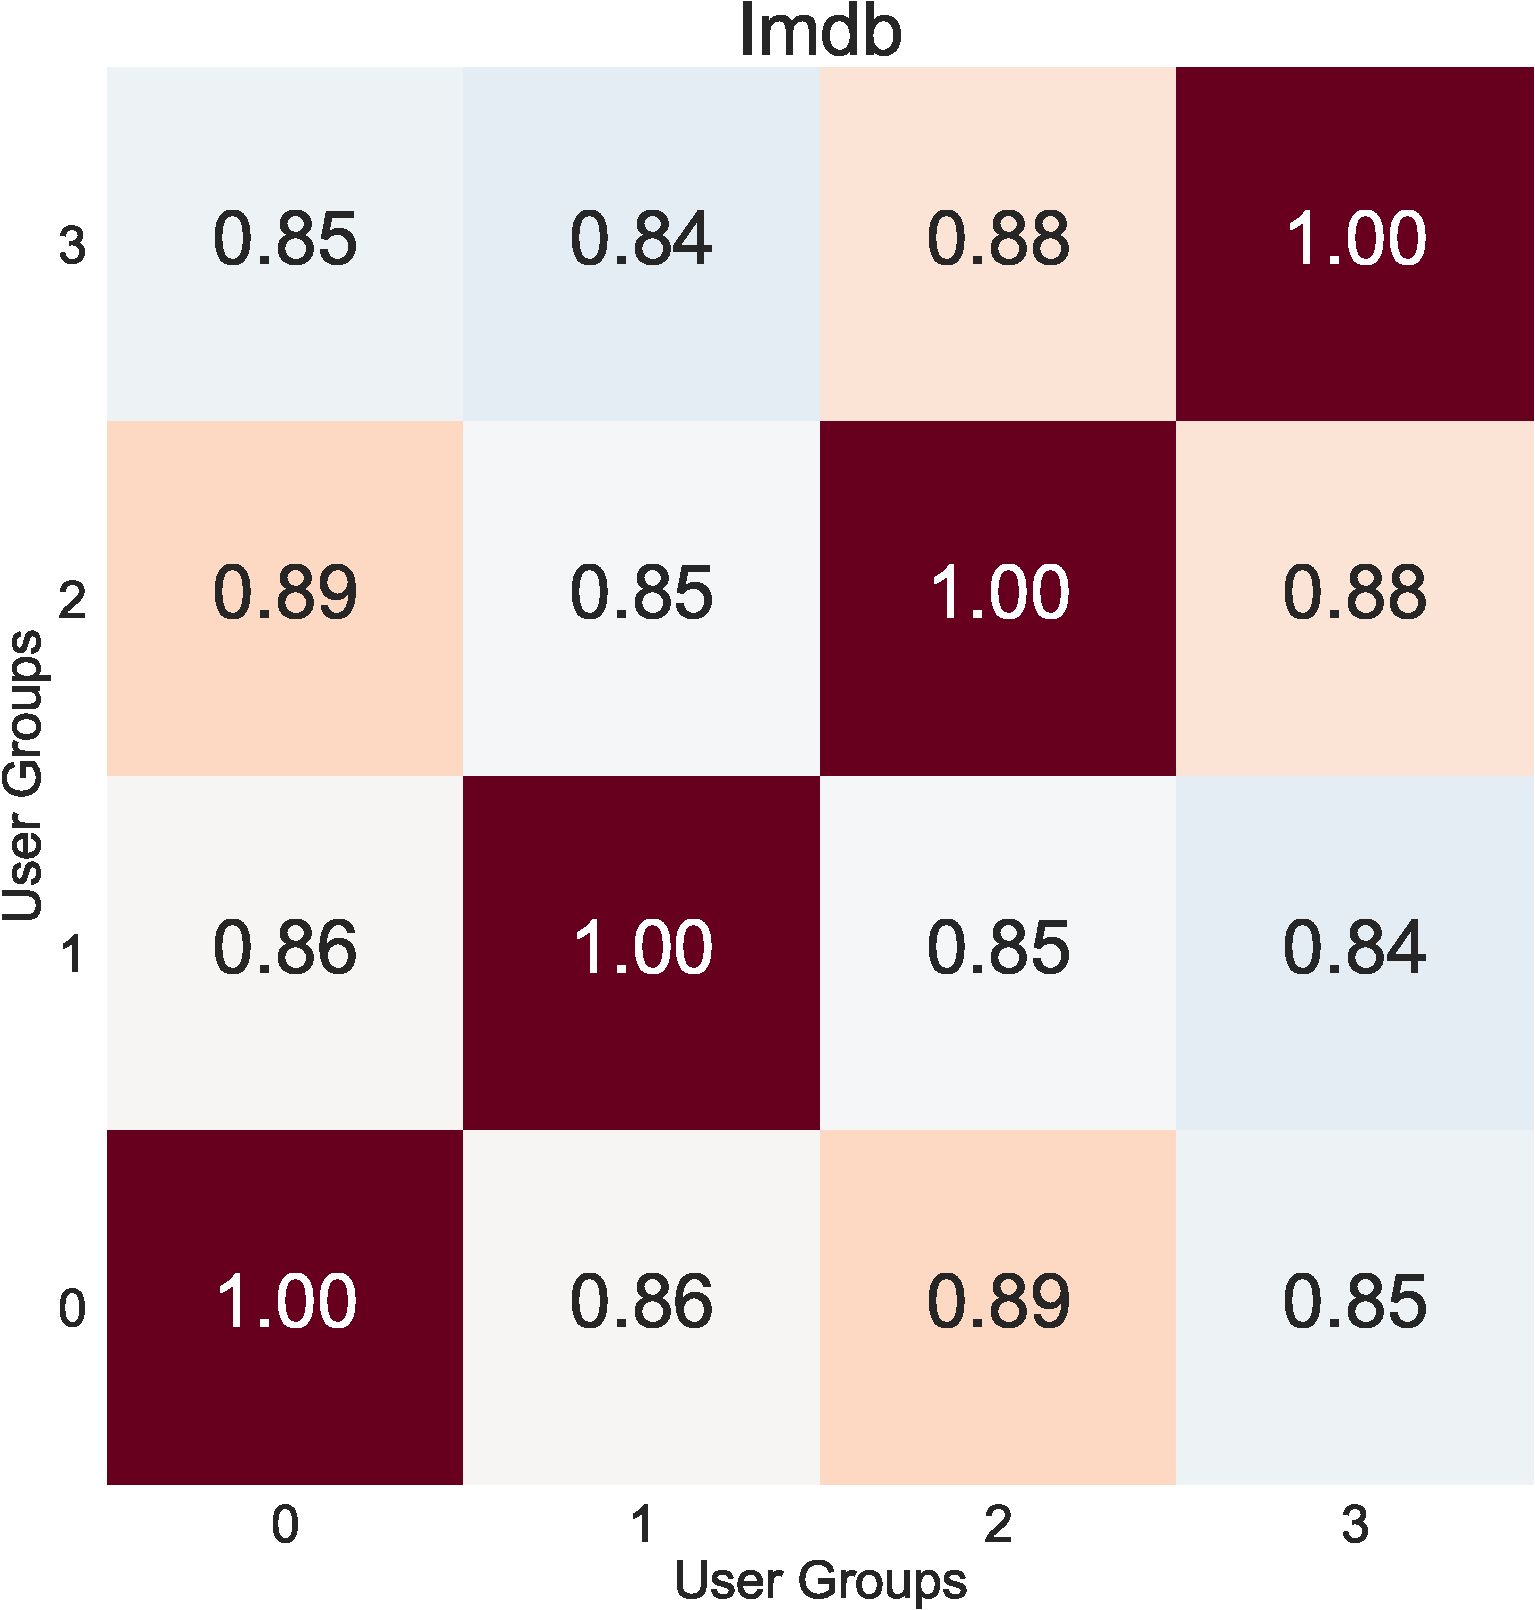
\includegraphics[width=0.325\textwidth]{./images/chapter4/uembedding/imdb_word.pdf}
    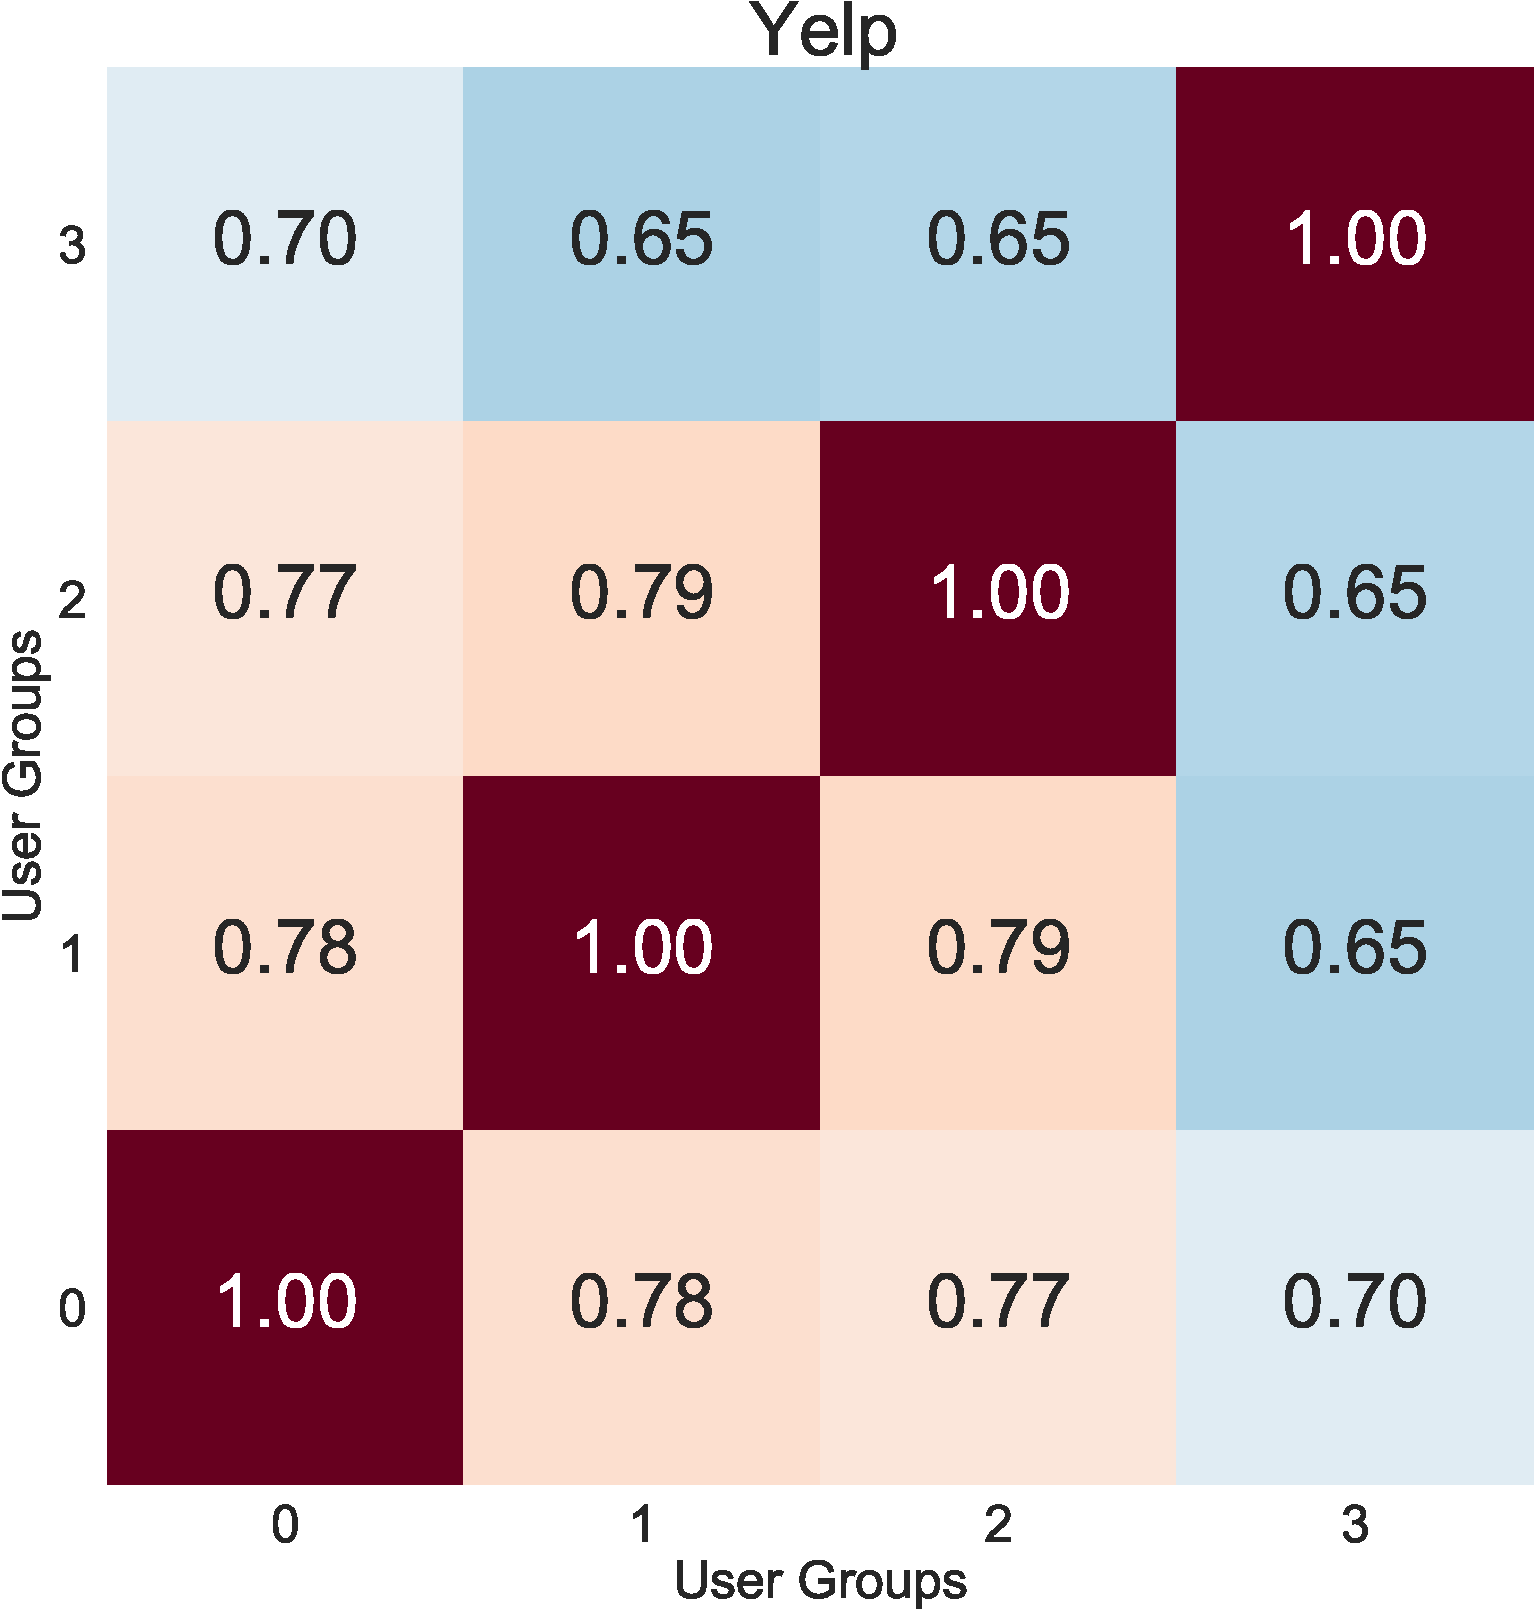
\includegraphics[width=0.325\textwidth]{./images/chapter4/uembedding/yelp_word.pdf}
    \caption{Word feature overlaps between every two user groups. A value of 1 means no variations of top features between two user groups, while values less than 1 indicate more feature variations.}
    \label{chap4:fig:word_user}
\end{figure*}


Existing methods mainly infer user embeddings from features of text contents~\cite{pan2019social}.
Therefore, word usage variations across the user interests will change word distributions and further impact the stability of user embeddings.
We aim to test whether there are language variations across the user interests in our datasets and how strong they are.

We consider word usage as it relates to user embeddings by estimating the overlap of top word features across the product genres, the types of reviewed products in Amazon, business units in Yelp and movies in IMDb.
To solve data sparsity caused by single user preference, we grouped users and therefore their generated documents according to genres of user-reviewed products.
We refer to this as genre domains.
We build a unified feature vectorizer~\cite{pedregosa2011scikit} with TF-IDF-weighted $n$-gram features ($n \in \{1,2,3\}$), removing features that appeared in less than 2 documents.
We rank and select the top 1000 word features for each genre domain by mutual information.
We then compute the intersection percentage between every two genre domains: let $F_0$ is the set of top features for one genre domain and $F_1$ is the set of top features for the other domain, then the overlap is $|F_0 \cap F_1|/1000$.

We show the results in Figure~\ref{chap4:fig:word_user}.
The overlap varies significantly across genre domains. 
This indicates that the word usage and its contexts of users change across user interests and preferences. 
Since the training of user embeddings relies heavily on the language features of users, this suggests that it is important to consider the language variations in user interests for the user embeddings.


\subsubsection{Classification Performance Variations}

\begin{figure*}[t]
\centering
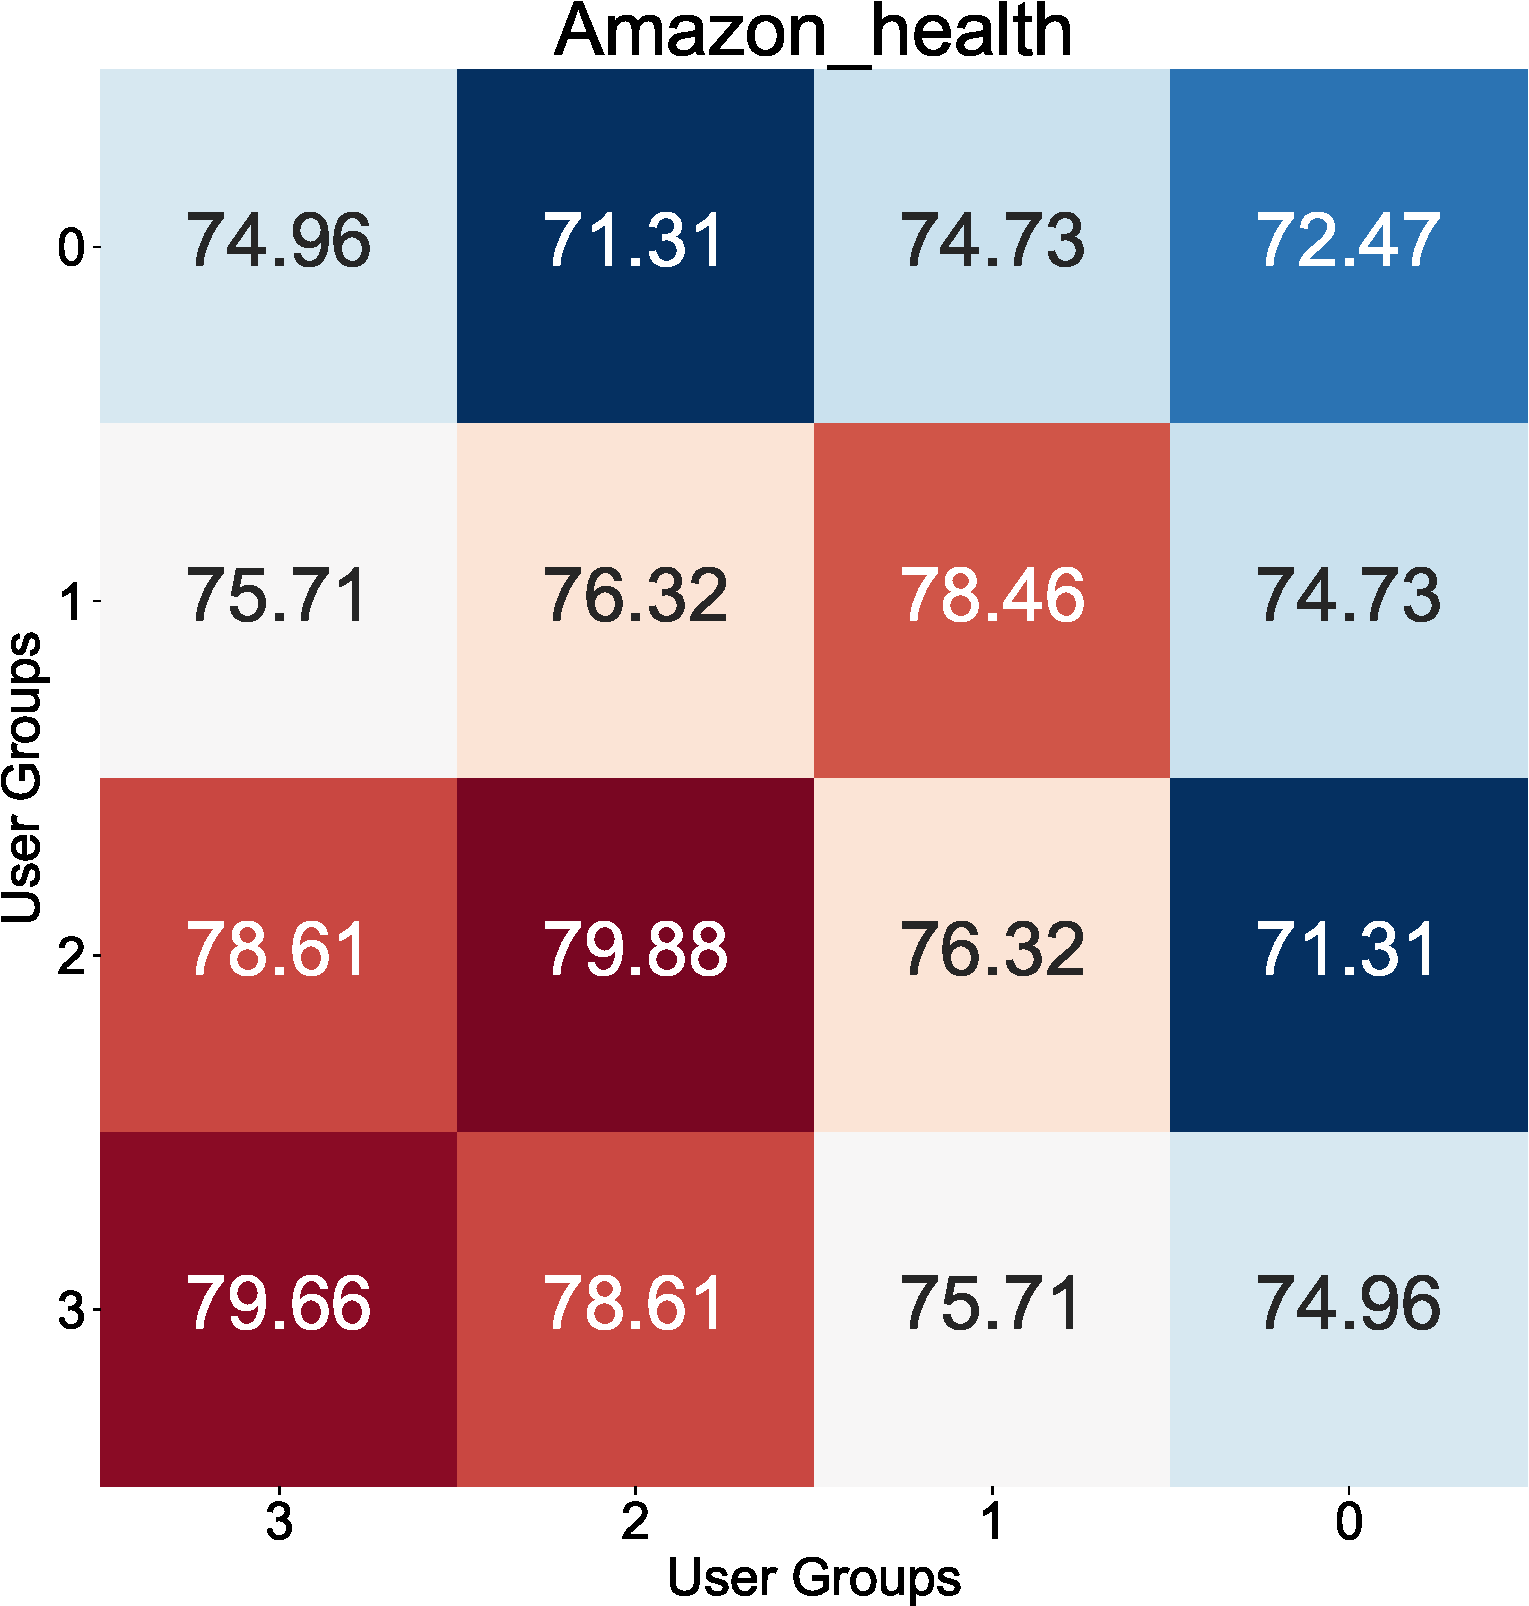
\includegraphics[width=0.325\textwidth]{./images/chapter4/uembedding/amazon_health_group.pdf}
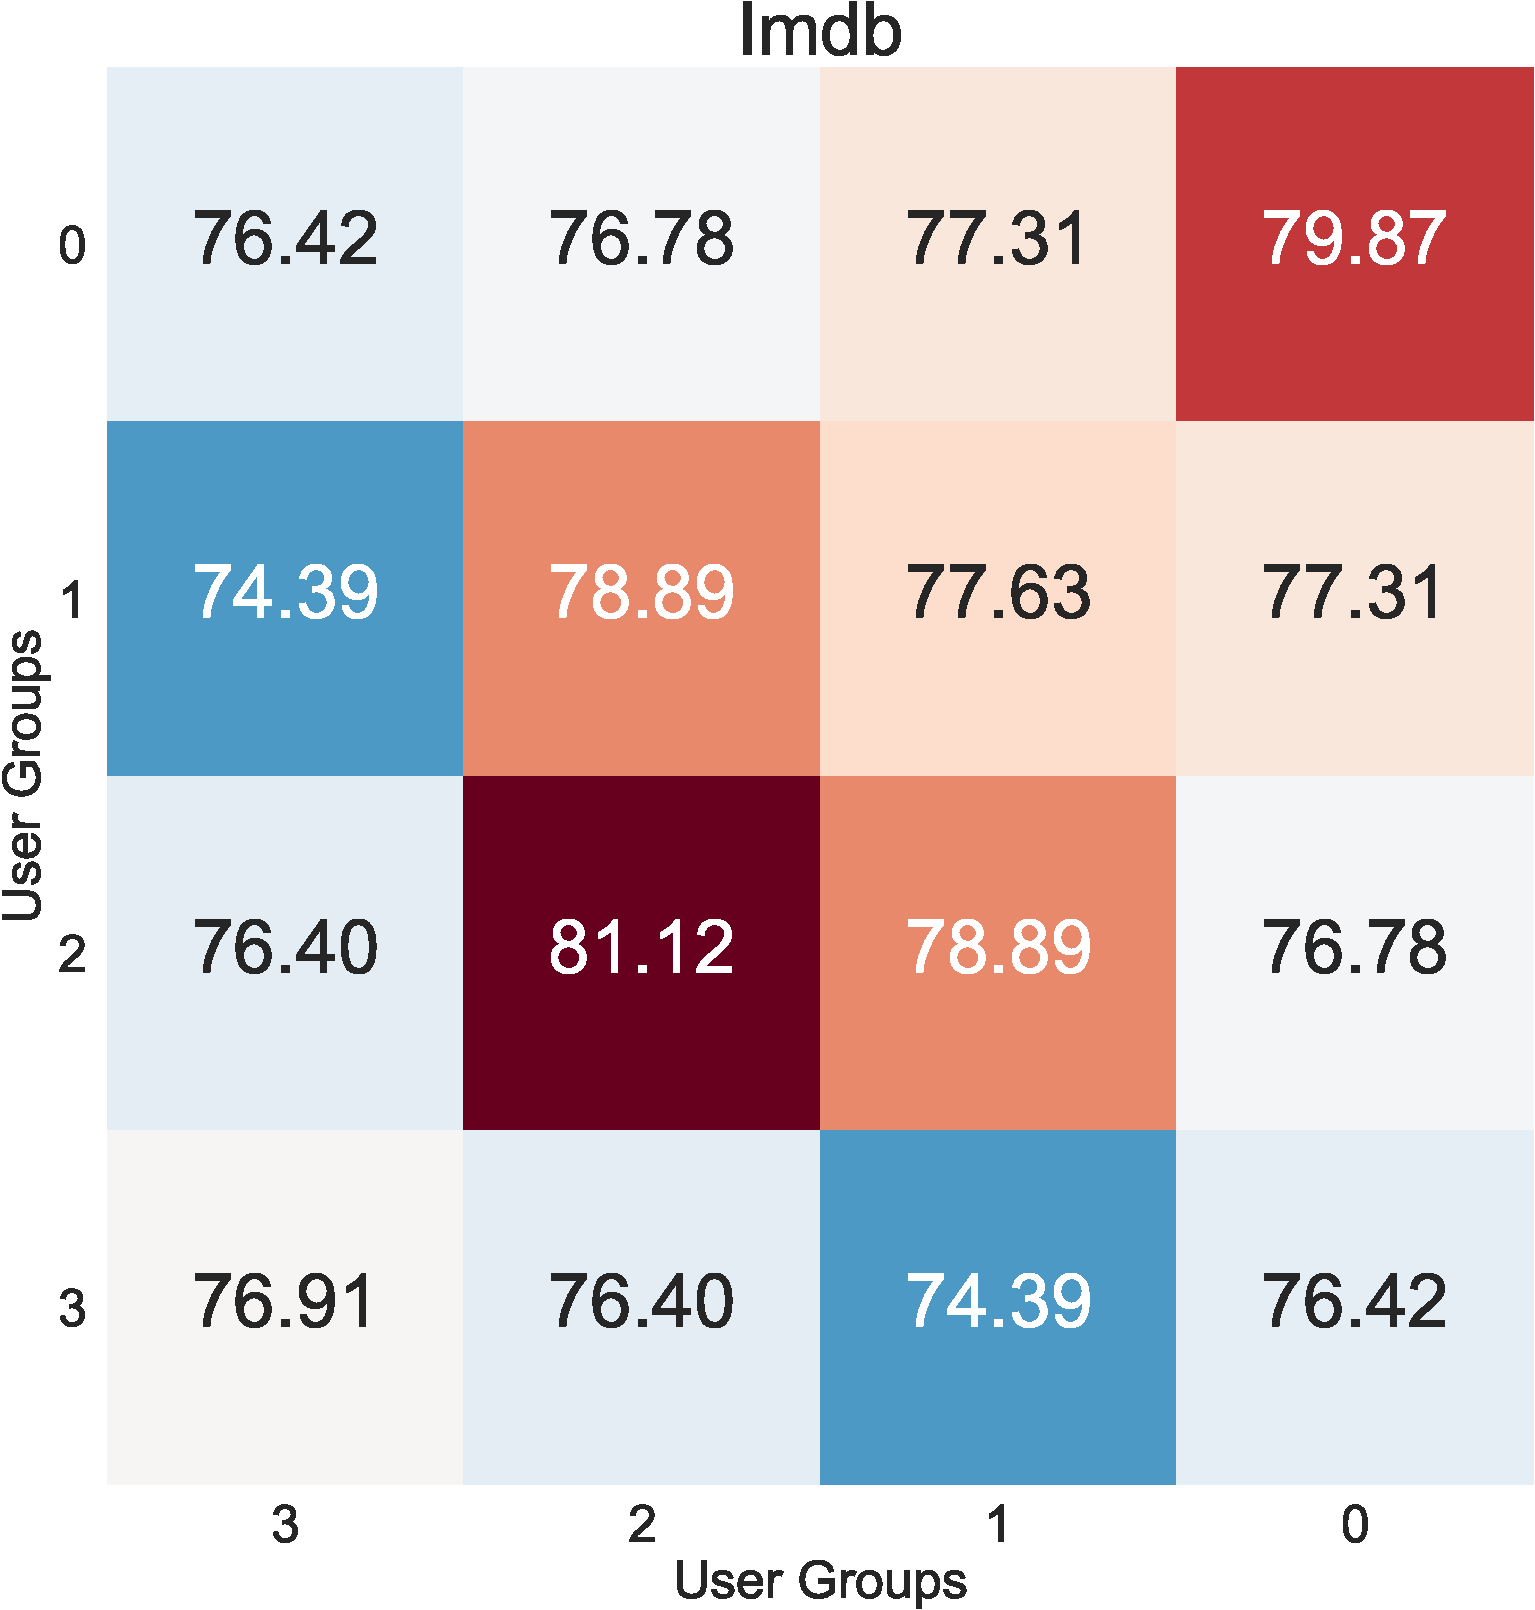
\includegraphics[width=0.325\textwidth]{./images/chapter4/uembedding/imdb_group.pdf}
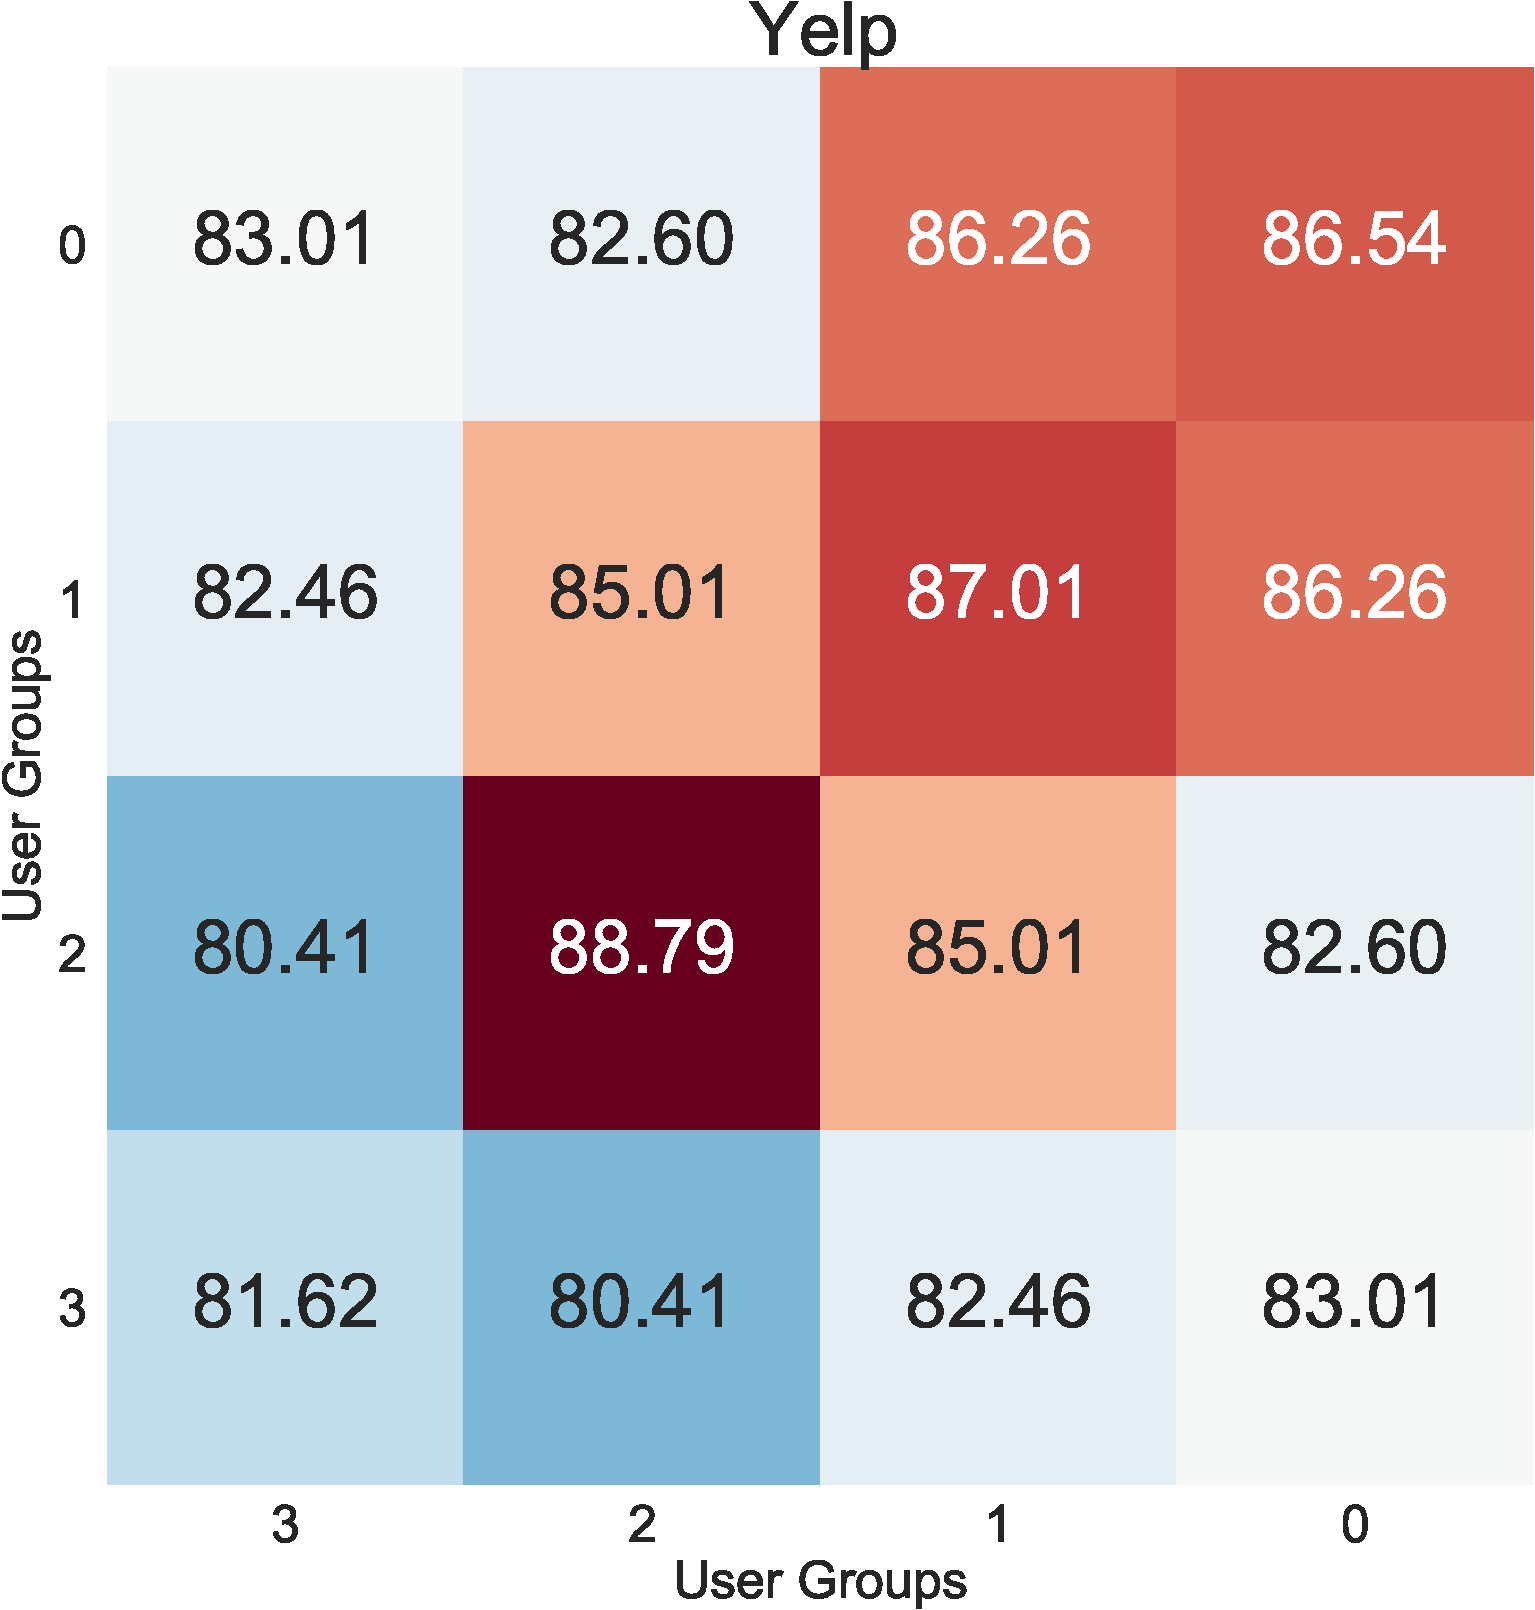
\includegraphics[width=0.325\textwidth]{./images/chapter4/uembedding/yelp_group.pdf}
\caption{Document classification performance when training and testing on different groups of users. The datasets come from Amazon health, IMDb and Yelp reviews. Darker red indicates better classification performance, while darker blue means worse performance.}
\label{chap4:fig:group}
\end{figure*}

User embeddings are effective to understand user behaviors in the classification setting~\cite{amir2016modelling, ding2018predicting}.
Research has found that combining user and document representations can benefit classification performance~\cite{yuan2019neural}.
We explore how language variations in user interests can affect classification models.

We analyze by training and testing classifiers that group users by the categories of reviewed products.
We first group products and users according to product genres, which can be treated as different user domains. 
For each domain, we downsampled the documents, users and products within each group to match the numbers in the smallest group, so that classification performance differences are not due to the data sizes.
For each grouped documents, we shuffle and split the data into training (80\%) and test (20\%) sets. We train logistic regression classifiers~\cite{pedregosa2011scikit} using TF-IDF-weighted uni-, bi- and tri-gram features. 
We report weighted F1 scores across grouped users and show the results in Figure~\ref{chap4:fig:group}.

Classification performance varies across the grouped users.
Higher performance variations between in- and out- user groups suggest higher user variations and vice versa.
The performance variations suggest that user behaviors vary across the categories of user interests. 
We can also observe that classification models generally perform better when tests within the same user groups while worse in the other user groups.
This suggests a variability connection between the user interests and language usage, which derives user embeddings. 



% \subsubsection{Analysis 3}

% \begin{figure}[htp]
% \centering
% 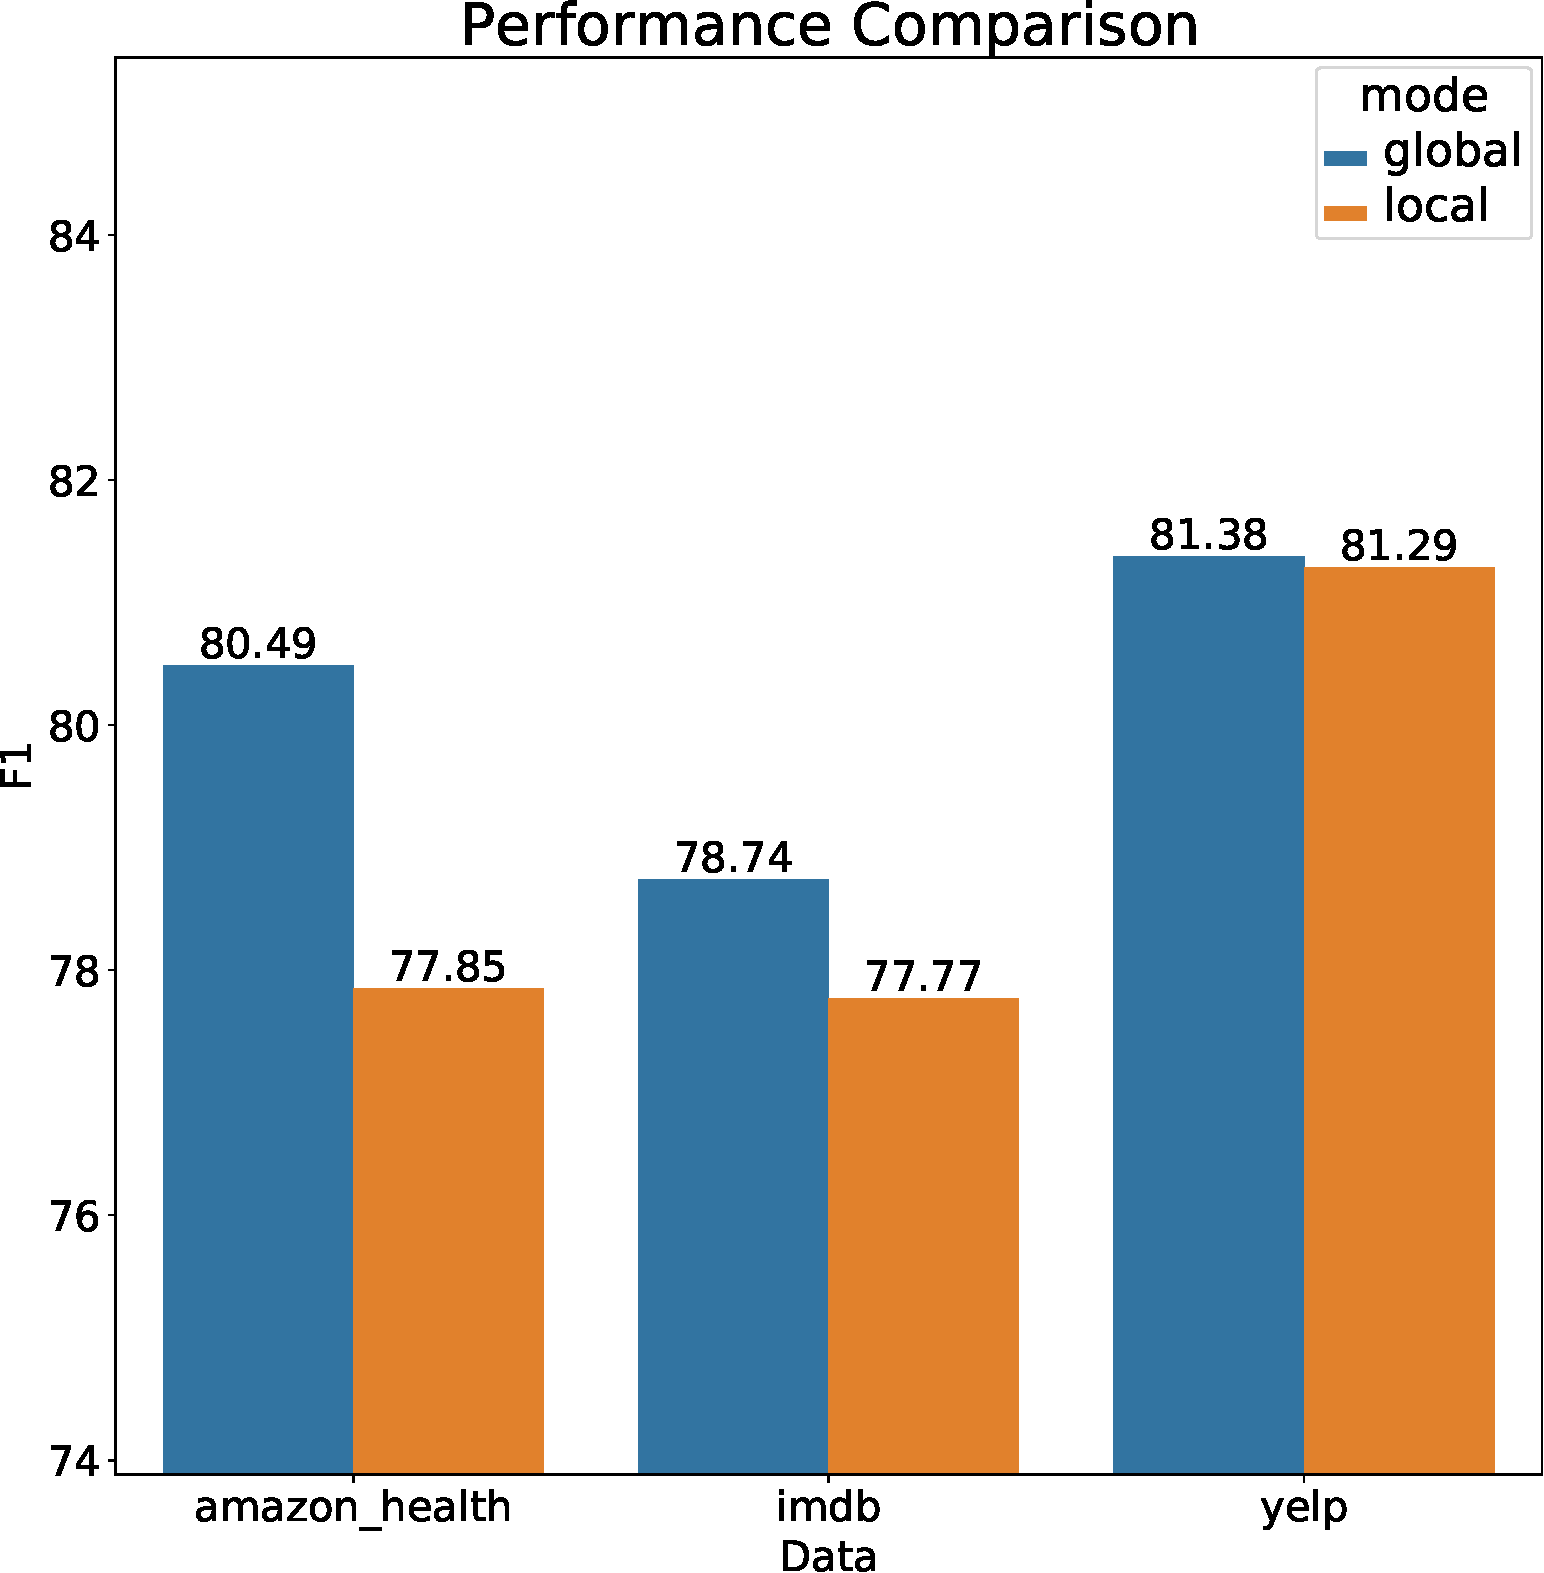
\includegraphics[scale=0.40]{./images/chapter4/uembedding/ctt_results.pdf}
% \caption{F1 scores of document classification performance when training models on different feature sets. The blue color indicates the classifier uses both local and global feature sets, while the orange one only uses local feature set.}
% \label{chap4:fig:global_local}
% \end{figure}

\subsection{Multitask User Embedding}
\label{chap4:subsec:model2}


\begin{figure*}[t!]
\centering
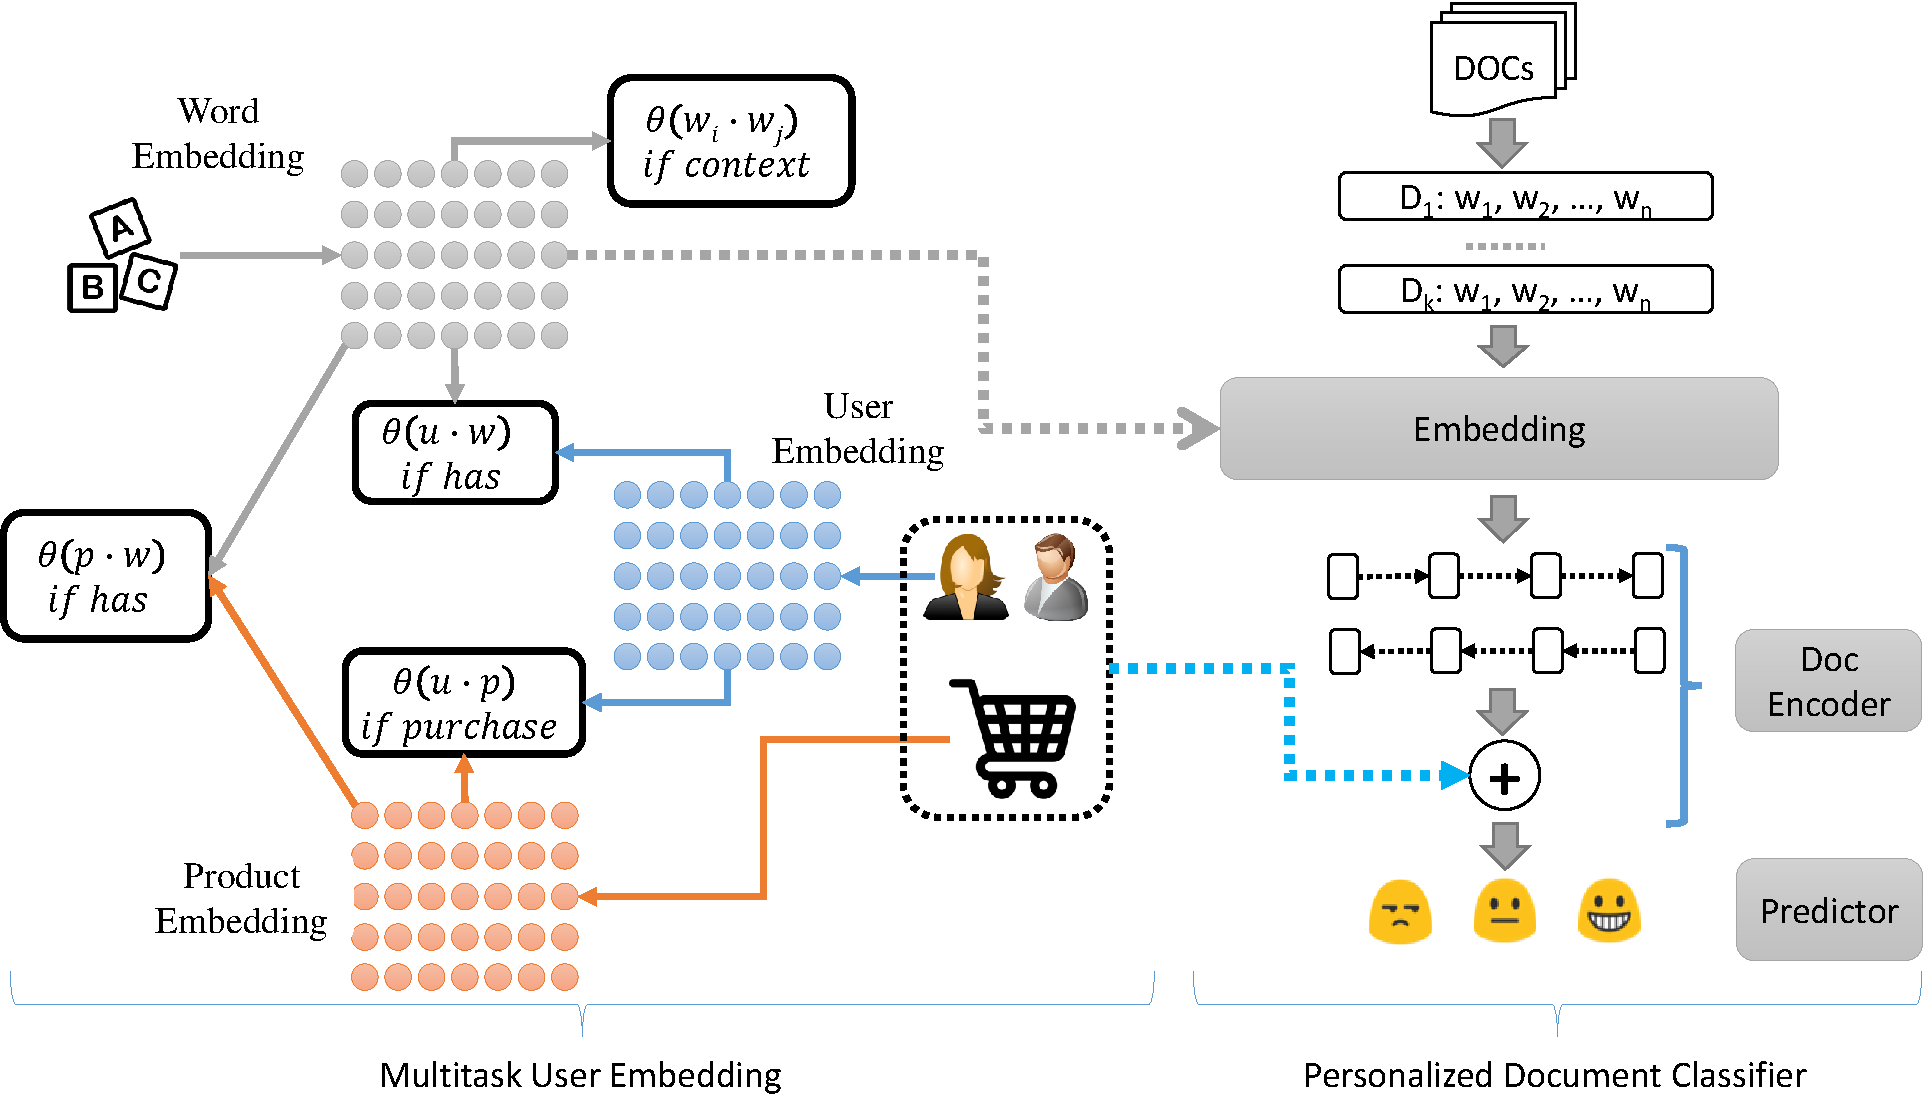
\includegraphics[width=1\textwidth]{./images/chapter4/uembedding/userEmbedding-diagram.pdf}
\caption{Illustrations of User Embedding via multitask learning framework on the left and personalized document classifiers using the trained embedding models on the right. The arrows and their colors refer to the input directions and input sources respectively. We use the logos of people, shopping cart and ABC to represent user, product and word inputs. The $\bigoplus$ is the concatenation operation of representations.}
\label{chap4:fig:uemb_diagram}
\end{figure*}

We present the architecture of the proposed model in Figure~\ref{chap4:fig:uemb_diagram} on the left.
Methods~\cite{pan2019social} to train text-based user embedding mainly focus on the user-generated documents while ignoring user factors, the user interests. 
A close work to ours only trained user embeddings by predicting if users co-occurred with sampled words~\cite{amir2017quantifying}.
We extend this line of work by adapting user interests, products and language usage into modeling steps.
The proposed unsupervised model trains four joint tasks based on the Skip-Gram~\cite{mikolov2013distributed}: word and word, user and word, product and word and user and product. 
Note that we do not use the categories of products and user interests in our training steps.
Then we can optimize the model by minimizing the following loss function: 

$\mathcal{L} = \mathcal{L}(w, w) + \mathcal{L}(u, w) + \mathcal{L}(p, w) + \mathcal{L}(p, u)$
where $w$, $u$, $p$ are the notations of words, users and products respectively.
Considering the large size of the vocabulary, users and products, we approximate our optimization objectives by the negative sampling.
Then we can treat each task as a classification problem and calculate loss values by the binary cross-entropy.
We present the details of each optimization task as following:
% We can represent the user, product, document, vocabulary sets as $U = \{u_1, ..., u_n, ..., u_N\}$, $P = \{p_1, ..., p_m, ..., p_M\}$, $D = \{d_1, ..., d_c, ..., d_C\}$ respectively, where the N, M and C are the set sizes. 
% Write math notations and equations.

\paragraph{Word and word}
is a standard way to train Word2vec~\cite{mikolov2013distributed} models. The prediction task is to predict if the sampled words have co-occurred within the window context. The training process uses negative sampling to approximate objective function. We choose 5 as the number of negative samples. We keep the top 20,000 frequent words and finally replace the rest of the words with the special token, $<unk>$. 


\paragraph{User and word}
predicts if a user authored the sampled words by the contexts of user posts. The goal is to learn patterns of user language usage from user historical posts. Given a document $i$, its author $u_i$ and the user's vocabulary $V_{u_i} = \{w_{1, i}, ..., w_{j, i}, ..., w_{n, i}\}$, where n is the number of frequent words authored by the user. Our objective is to minimize the following function:

$\mathcal{L}(u, w) = -\sum_{w_j \in V_{u_i} \\ w_k \in V \\ w_k \notin V_{u_i}}[log(\theta(e(u_i) \cdot e(w_j))) +  log(\theta(e(u_i) \cdot e(w_k)))]$
where $w_j$ is a negative sample from the whole vocabulary $V$, $e(u)$ and $e(w)$ are the fixed-length user and word vectors, and $\theta$ is a sigmoid function to normalize values of the dot production. We extend the previous work~\cite{amir2017quantifying} to integrate both local and global user language usage by sampling $w_j$ from a combined token list of both the input document and the user's vocabulary.
This can help the model learn contextual information of the user.


\paragraph{Product and word}
follows the prediction task of user and word to classify if sampled words describe the selected product. This task is to use the contents generated by users to train the representations of products. Then we can have 

$\mathcal{L}(p, w) = -\sum_{w_j \in V_{p_i}, w_k \in V, w_k \notin V_{p_i}}log(1 - \theta(e(p_i) \cdot e(w_j))) + log(\theta(e(p_i) \cdot e(w_k)))$
where $V_{p_i}$ is the vocabulary of the product $p_i$ and $w_k$ is a negative sample of words.
The language can be viewed as a bridge between the interactive relation of user and product, which predicts language usage for both products and users.


\paragraph{User and product}
learns if a user commented on the sampled products. The prediction task aims to adapt product-related latent factors into the user embeddings.
Given a document $i$, its author $u_i$ and the reviewed product $p_i$,
we can optimize the task by minimizing

$\mathcal{L}(u, p) = -\sum_{p_k \in P, p_k \notin P_{u_i}}log(\theta(e(p_i) \cdot e(u_i))) + log(\theta(e(p_k) \cdot e(u_i)))$
where the $P$ is the collection of all products, the $P_{u_i}$ is the reviewed products of the user and the $p_k$ is a negative sample that the user does not purchase the product.
The constraints between products and users can help user embeddings discriminate language variations across the product domains.
The relation of user and product can also personalize product vectors.

For model settings, we used Adam~\cite{kingma2014adam} for the model optimization with a learning rate of 1e-5. We set the training epochs as 5. The model initializes embedding vectors randomly and learns 300-dimension representations for words, users and products. We empirically use 5 as the number of negative samples. For the other parameters, we keep the same as the defaults in the Keras~\cite{chollet2015keras}. 


\subsection{Experiments}
\label{chap4:subsec:exp2}

We evaluate the effectiveness of the user factor adapted embedding model by an intrinsic evaluation, user clustering task and an extrinsic evaluation, personalized classification task. The first task aims to measure the purity of clusters with respect to categories of user interests, and the second task uses the document classification as a proxy of qualifying quality of user embeddings. We conduct a qualitative analysis of the user embeddings comparing with the close work~\cite{amir2017quantifying}.


\subsubsection{User Clustering Evaluation}

The unsupervised evaluation of embedding models focuses on four main categories: relatedness, analogy, categorization and selectional preference~\cite{schnabel2015evaluation}.
We approach the user embedding evaluation by categorizing users into different clusters. 
User communities or groups gather users by their interests and behaviors, such as engaging in the same field of topics~\cite{benton2016learning, yang2017overcoming}.
In our datasets, the user-purchased products, the user-visited business units and the user-watched movies have their product categories. 
The categories can imply user preferences and interests, and therefore can help evaluate user clusters.
In this study, our proposed multitask model learns interactive relations across language, user and product instead of using the product categories. We compare our proposed model with other 5 baseline models:

\paragraph{word2user} 
represents users by aggregating word representations~\cite{benton2016learning}. We compute a user representation by averaging embeddings of all tokens that were authored by the user. To obtain the word embeddings, for each dataset, we trained a word2vec model for 5 epochs using Gensim~\cite{rehurek2010software} with 300-dimensional vectors.


\paragraph{lda2user} 
generates user representations by applying Latent Dirichlet Allocation (LDA)~\cite{blei2003latent} on user documents~\cite{pennacchiotti2011machine}. We set the number of topics as 300 and leave the rest of the parameters as their defaults in  Gensim~\cite{rehurek2010software}. We apply the LDA model on each user document to obtain a document vector, and then get a user vector by averaging the vectors of all the user's documents.


\paragraph{doc2user} 
applies paragraph2vec~\cite{le2014distributed} to obtain user vectors. We implemented the User-D-DBOW model which achieved the best performance in the previous work~\cite{ding2017multi}. The implementation keeps parameters with default values in the Gensim~\cite{rehurek2010software}. We aggregate each user's documents as a single document. Then the User-D-DBOW model can derive a single user vector from the aggregated document.

\paragraph{bert2user} 
follows a similar process of the lda2user. We use the ``bert-base-uncased'' pre-trained BERT model
for English from the transformers toolkit~\cite{Wolf2019HuggingFacesTS} with default parameter and model settings. After inserting ``[CLS]'' and ``[SEP]'' to the beginning and end of each document, the BERT model encodes a document into a fixed-length (768) document vector. We can then generate user embeddings by averaging each user's all document vectors.


\paragraph{user2vec} trains user embeddings by predicting word usage by users.
We follow the existing work~\cite{amir2017quantifying} but set the user vector dimension as 300.


\begin{table*}[htp]
\centering
\resizebox{\textwidth}{!}{
    \begin{tabular}{cc||ccc|ccc|ccc}
    \multicolumn{2}{c||}{\multirow{2}{*}{}} & \multicolumn{3}{c|}{Amazon-Health} & \multicolumn{3}{c|}{IMDb} & \multicolumn{3}{c}{Yelp} \\
    \multicolumn{2}{c||}{} & F1@4 & F1@8 & F1@12 & F1@4 & F1@8 & F1@12 & F1@4 & F1@8 & F1@12 \\\hline\hline
    \multirow{5}{*}{Baselines} & word2user & \textbf{.929} & .909 & .905 & .653 & .725 & .762 & .859 & .810 & .797 \\
     & lda2user & .920 & \textbf{.914} & .900 & .696 & .726 & .761 & .849 & .839 & .832 \\
     & doc2user & .873 & .891 & .901 & .660 & .725 & .748 & .836 & .828 & .826 \\
     & bert2user & .871 & .896 & \textbf{.906} & .660 & .714 & .734 & .838 & .828 & .830 \\
     & user2vec & .868 & .891 & .901 & .601 & .600 & .593 & .841 & .829 & .832 \\\hline
     
    Ours & MTL & .870 & .890 & .900 & \textbf{.801} & \textbf{.879} & \textbf{.884} & \textbf{.879} & \textbf{.843} & \textbf{.838} 
    % \multirow{3}{*}{Ours} & MTL-global &  &  &  &  &  &  &  &  &  \\
    %  & MTL-decay &  &  &  &  &  &  &  &  &  \\
    %  & MTL-local &  &  &  &  &  &  &  &  & 
    \end{tabular}
}
\caption{Performance summary of different user embedding models. We report F1 scores at multiple numbers of clusters. The bold fonts indicate the best performance in each evaluation task.}
\label{chap4:tab:usereval}
\end{table*}


We use the \texttt{SpectralClustering} algorithm from the scikit-learn~\cite{pedregosa2011scikit} toolkit to cluster users into three clustering sizes, 4, 8 and 12. 
We set the affinity as cosine and leave other parameters as their defaults.
To measure the cluster quality, we select every two users from the clusters without repetition.
We count the user pair as a correct option if the two users have overlaps within the same product genre and from the same cluster or if the user pair does not overlap and is from the different clusters.
Otherwise, we will count the selection as the wrong option.
Therefore, we can have a list of predicted labels and ground truths by using the product genres as a proxy.
Finally, we measure the clustering purity by the F1 score.

We present results at Table~\ref{chap4:tab:usereval}.
The results show that the multitask user embedding model outperforms the other baselines by a large portion on the IMDb and Yelp datasets.
The improvements suggest the user factor adapted model can understand semantic variations in diverse user interests.
The performance of our model and user2vec have similar scores on the Amazon-Health dataset.
Comparing to the other two datasets, the Amazon-Health data has more similar topics of products.


\subsubsection{Personalized Classifier Evaluation}

We train three classifiers to evaluate user embeddings on the document classification task.
We split each dataset into training (80\%), development (10\%) and test (10\%) sets, as shown in Table~\ref{chap4:tab:data2}. 
The models oversample the minority during the training process.
We test the classifiers when they achieve the best performance on the development set.
Finally, we report precision, recall and F1 scores using the \texttt{classification\_report} from scikit-learn~\cite{pedregosa2011scikit}.
Figure~\ref{chap4:fig:uemb_diagram} illustrates personalizing classifiers by concatenating document representations with user embeddings.
We compare our proposed model with classifiers using existing user2vec~\cite{amir2017quantifying} and non-personalized classifiers.
To ensure a fair comparison, classifiers use the same settings for models with and without user embeddings.

\paragraph{LR.}
We build a logistic regression classifier using \texttt{LogisticRegression} from scikit-learn \cite{pedregosa2011scikit}. The classifier extracts uni-, bi- and tri-gram features on the corpora with the most frequent 15K features with default parameters. 


\paragraph{GRU.} 
We build a bi-directional Gated Recurrent Unit (GRU)~\cite{cho2014properties} classifier. We padded documents to the average document length of each corpus. We set the output dimension of GRU as 200 and apply a dense layer on the output. The dense layer uses ReLU~\cite{hahnloser2000digital} as the activation function, applies a dropout~\cite{srivastava2014dropout} rate of 0.2 and outputs 200 dimensions for final document class prediction. We train the classifier for 20 epochs.


\paragraph{BERT.} 
We implement a BERT-based classifier by HuggingFace's transformers toolkit \cite{Wolf2019HuggingFacesTS}. The classifier loads the ``bert-base-uncased'' pre-trained BERT model for English, encodes each document into a fixed-length (768) vector and feeds to a linear prediction layer for prediction.  We conduct fine-tuning steps for 10 epochs with a batch size of 32 and optimize the model by \texttt{AdamW} with a learning rate of 9$e^{-5}$. 



\begin{table*}[t]
\centering
\begin{tabular}{c||ccc|ccc|ccc}
\multirow{2}{*}{Methods} & \multicolumn{3}{c|}{Amazon-Health} & \multicolumn{3}{c|}{IMDb} & \multicolumn{3}{c}{Yelp} \\
 & Precision & Recall & F1 & Precision & Recall & F1 & Precision & Recall & F1 \\\hline\hline
LR & .834 & .768 & .793 & .818 & .779 & .794 & .856 & .820 & .833 \\
LR-u & .841 & .777 & \textbf{.801} & .834 & .791 & \textbf{.807} & .860 & .821 & .835 \\
LR-up & .838 & .771 & .796 & .833 & .791 & \textbf{.807} & .863 & .825 & \textbf{.838} \\\hline
GRU & .813 & .844 & .812 & .824 & .837 & .823 & .851 & .865 & .852 \\
GRU-u & .836 & .811 & .821 & .832 & .819 & .825 & .868 & .846 & .858 \\
GRU-up & .821 & .832 & \textbf{.825} & .846 & .824 & \textbf{.836} & .876 & .864 & \textbf{.867} \\\hline
BERT & .866 & .822 & .840 & .852 & .809 & .826 & .866 & .825 & .840 \\
BERT-u & .863 & .812 & .831 & .858 & .818 & .833 & .872 & .843 & \textbf{.854} \\
BERT-up & .873 & .838 & \textbf{.851} & .864 & .831 & \textbf{.844} & .880 & .839 & \textbf{.854}
\end{tabular}
\caption{Performance scores of document classifiers on the review datasets. `-u` means personalized classifiers using user2vec~\cite{amir2017quantifying} and `-up` indicates personalizing classifiers via our proposed method. We use the bold fonts to highlight the best performance of each classifier on separate datasets.}
\label{chap4:tab:personalization}
\end{table*}


We show the performance results in Table~\ref{chap4:tab:personalization}. Comparing to the baselines, the classifiers personalized by our proposed model generally achieve the best performance across the three datasets. 
This highlights adapting the user factor can help embedding models learn user variations and benefit classification performance on our datasets.
We can also observe that the personalized classifiers generally outperform the non-personalized classifiers.
This indicates personalizing the classifiers with user history boosts classification performance in our study.



\subsection{Visualization Analysis}

\begin{figure*}[t!]
\centering
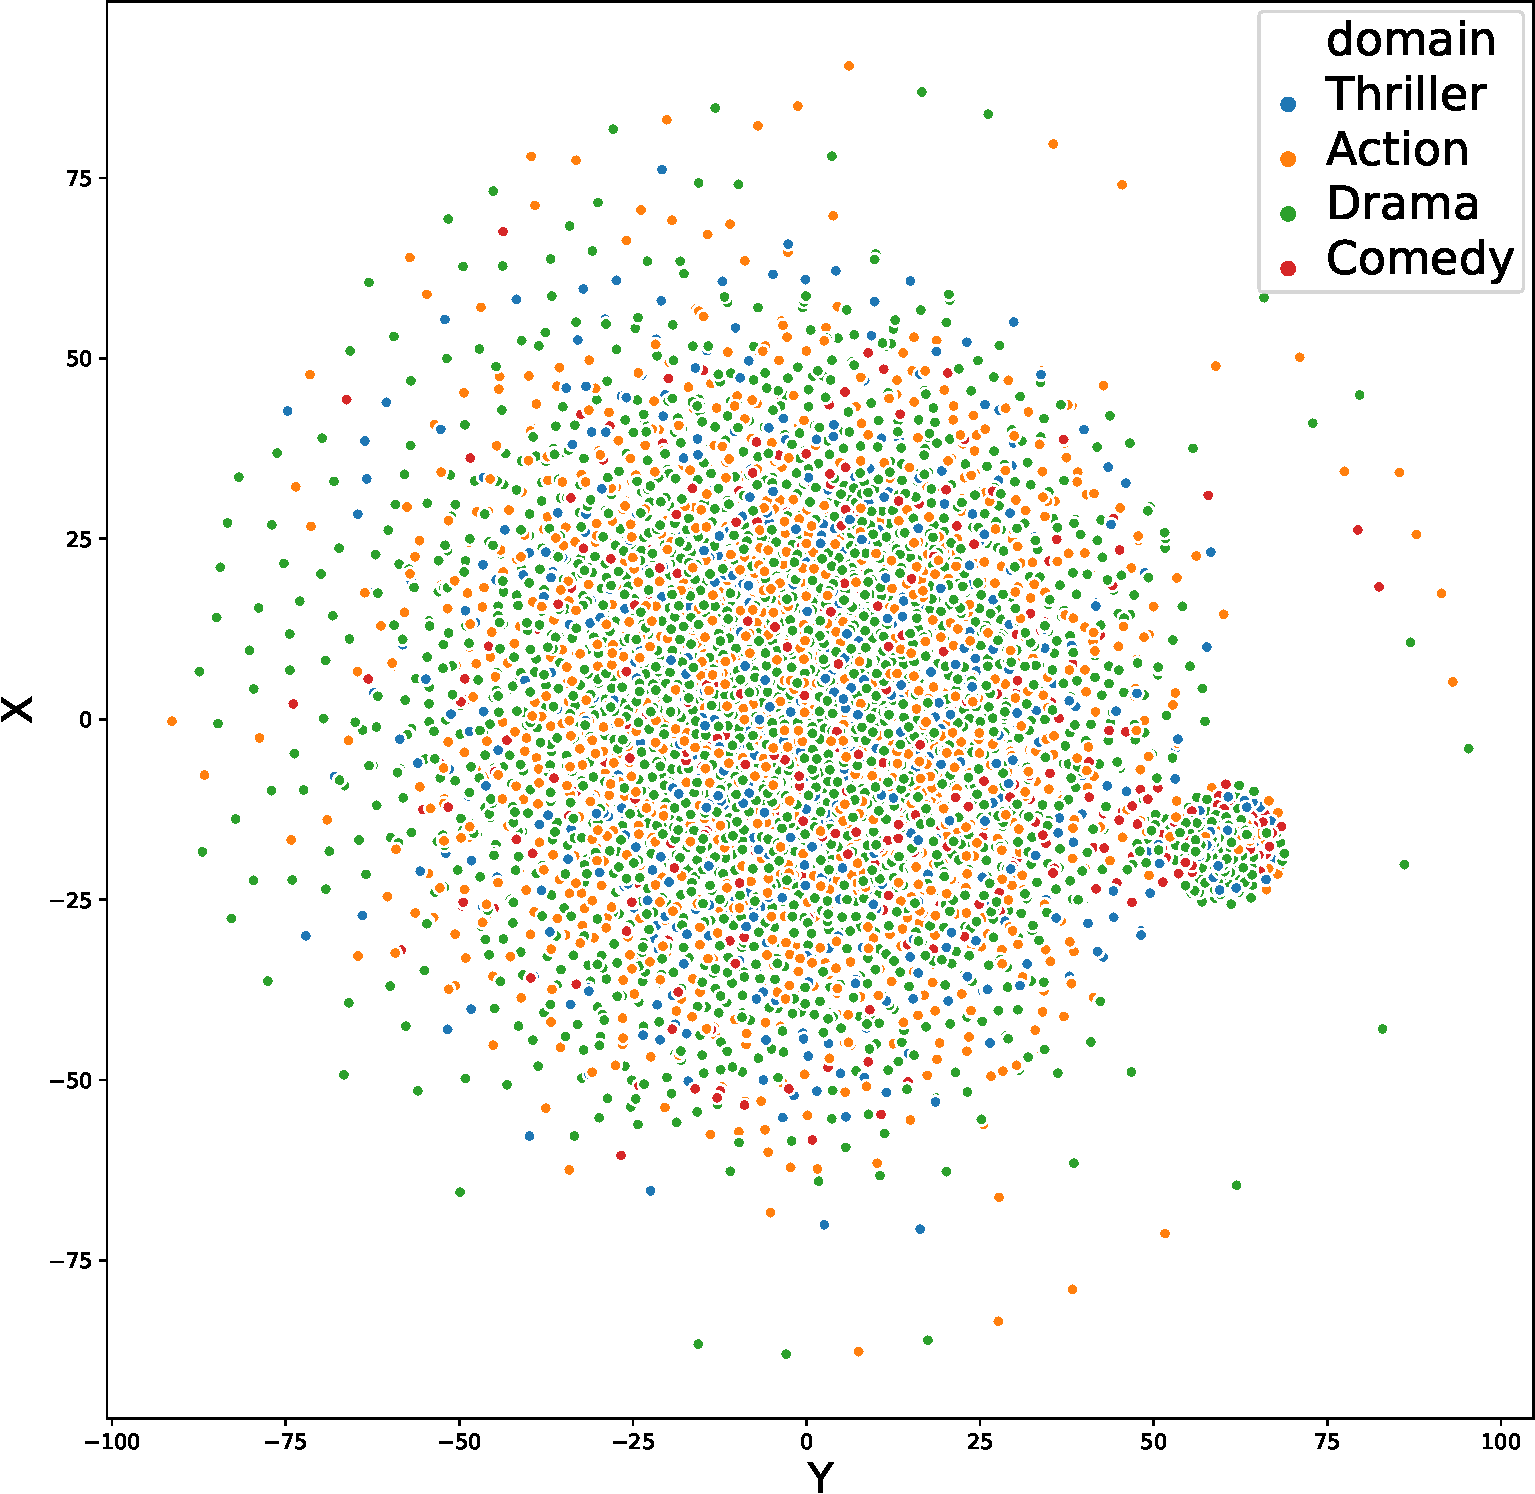
\includegraphics[width=0.495\textwidth]{./images/chapter4/uembedding/user2vec_emb_viz.pdf}
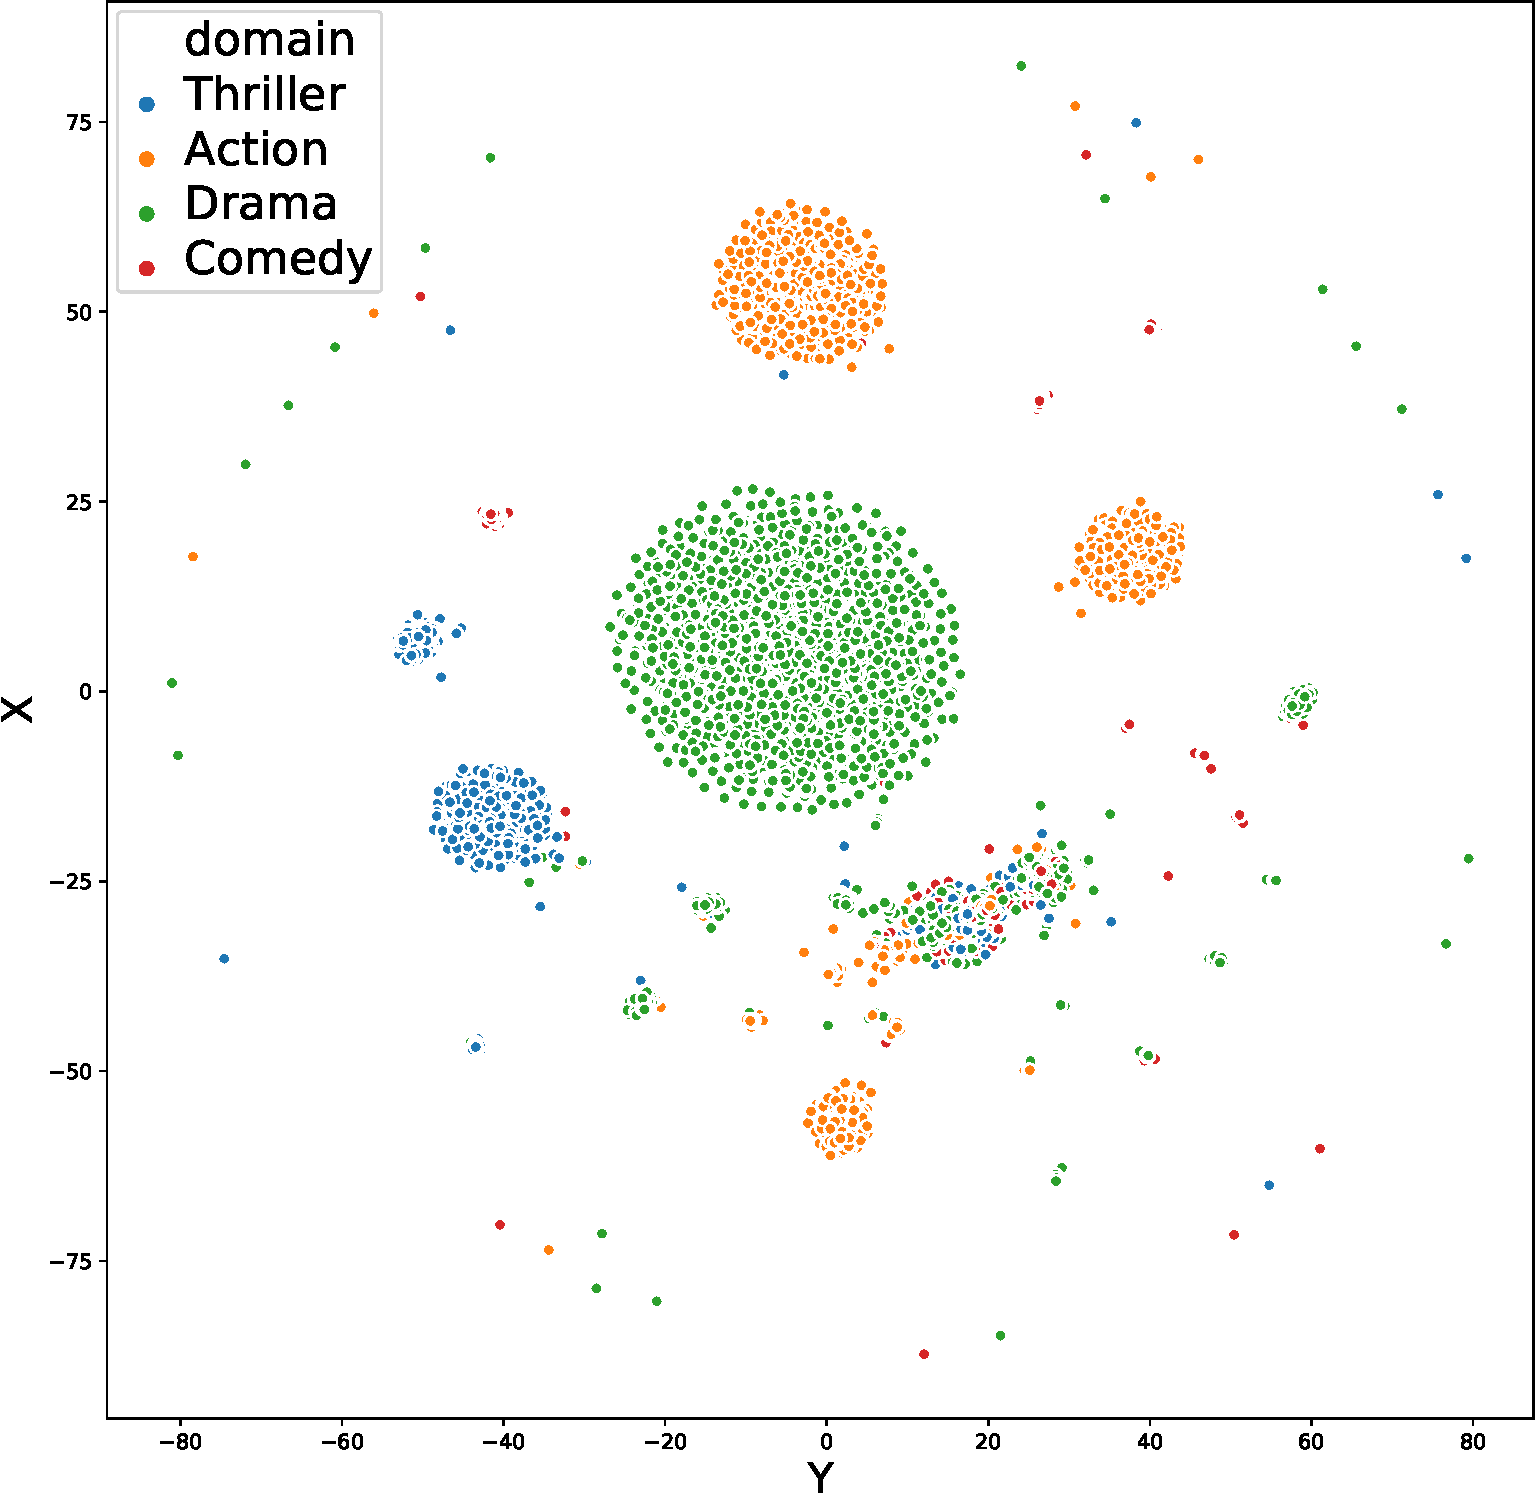
\includegraphics[width=0.495\textwidth]{./images/chapter4/uembedding/ours_emb_viz.pdf}
\caption{Visualizations of IMDb users colored concerning their interests in 4 movie genres. We plot users using the embeddings from our proposed method (right) and user2vec~\cite{amir2017quantifying} (left).}
\label{chap4:fig:uemb_viz}
\end{figure*}

To further evaluate the effectiveness of user embedding models, we map users into a 2-D space using user embeddings and plot them in Figure~\ref{chap4:fig:uemb_viz}.
We group users according to user interests using the domain categories of products.
To map the 300-d user embeddings, we use the \texttt{TSNE} algorithm from scikit-learn~\cite{pedregosa2011scikit} to compress the dimension into 2-d vectors. We set the n\_component as 2 and leave the other parameters as their defaults in the TSNE.
We can observe that the MTL user embedding model shows more clustering patterns with regard to user interests (product categories).
This indicates that the unsupervised multitask learning framework can adapt the latent user factors into the user embedding.
Users may have multiple interests. In the right plot, we can also find that there is a cluster that mixes with multiple colors on the right bottom.


\section{Conclusion}

In this chapter, we have explored user factor adaptation from two perspectives, demographic attributes and user interests.
We presented two major approaches for the user factor adaptation under the multitask learning framework, neural user demographic adaptation and multitask user embedding.
The experiments showed that various domain adaptation methods can be used to build classifiers that are more robust to demographics, combined in a neural model that outperformed prior approaches.
Our quantitative and qualitative analysis shows how user factors can cause user semantic variations in relation to word usage, topic shift and document classification, showing user factors are encoded in language.
The results suggest that the domain adaptation methods can boost classifiers and user embeddings that are more robust to language variations across user factors.
We publish our datasets\footnote{\url{http://cmci.colorado.edu/~mpaul/files/starsem2019_demographics.data.zip}} and source code.\footnote{Demographic factor adaptation: \url{https://github.com/xiaoleihuang/NUFA}. Multitask user embedding: \url{https://github.com/xiaoleihuang/UserEmbedding}.}

Our work in user factor adaptation highlights several future interesting directions to explore.
First, while our work is not focused specifically on reducing demographic biases,
our datasets, which contain various demographic attributes, could be useful in other research. 
This motivates us examine the demographic biases of document classifiers in the following Chapter~\ref{chp:fairness}. 
Second, user embedding models latent user factors inferred from user posts. A combination of user embedding and demographic attributes will help user embeddings better identify user semantic variations. 
Third, we have demonstrated language shift over time in Chapter~\ref{chp:temporality} and our proposed user embedding does not explicitly consider the temporal factor. An interesting future direction is to further explore the dynamic user embedding, which jointly models temporality and user behaviors.
